\documentclass[conference]{IEEEtran}
\IEEEoverridecommandlockouts
\usepackage{cite}
\usepackage{amsmath,amssymb,amsfonts,amsthm}
\usepackage{graphicx}
\usepackage{xcolor}
\usepackage{booktabs}
\usepackage{array}
\usepackage{multirow}
\usepackage{microtype}
\usepackage{enumitem}
\usepackage{url}
\usepackage[hidelinks]{hyperref}
\newtheorem{definition}{Definition}
\newtheorem{proposition}{Proposition}
% generated by paper/gen_numbers.py from reports/*.json -- do not edit
\providecommand{\missing}[1]{\textbf{\textcolor{red}{??#1}}}
\newcommand{\nAnchorAccactionitem}{81}
\newcommand{\nAnchorAccentitycount}{53}
\newcommand{\nAnchorAccquestion}{68}
\newcommand{\nAnchorAccsentiment}{82}
\newcommand{\nAnchorAcctopic}{52}
\newcommand{\nCalCtxQfourabs}{+3.6}
\newcommand{\nCalCtxQfourhi}{0.877}
\newcommand{\nCalCtxQfourlo}{0.402}
\newcommand{\nCalCtxQfourmed}{0.488}
\newcommand{\nCalCtxQoneabs}{+7.7}
\newcommand{\nCalCtxQonehi}{0.469}
\newcommand{\nCalCtxQonelo}{0.176}
\newcommand{\nCalCtxQonemed}{0.351}
\newcommand{\nCalCtxQthreeabs}{+3.8}
\newcommand{\nCalCtxQthreehi}{0.713}
\newcommand{\nCalCtxQthreelo}{0.207}
\newcommand{\nCalCtxQthreemed}{0.468}
\newcommand{\nCalCtxQtwoabs}{+17.1}
\newcommand{\nCalCtxQtwohi}{0.488}
\newcommand{\nCalCtxQtwolo}{0.242}
\newcommand{\nCalCtxQtwomed}{0.324}
\newcommand{\nCalParaBQfourabs}{-0.1}
\newcommand{\nCalParaBQfourhi}{0.062}
\newcommand{\nCalParaBQfourlo}{0.017}
\newcommand{\nCalParaBQfourmed}{0.024}
\newcommand{\nCalParaBQoneabs}{+11.9}
\newcommand{\nCalParaBQonehi}{0.706}
\newcommand{\nCalParaBQonelo}{0.374}
\newcommand{\nCalParaBQonemed}{0.564}
\newcommand{\nCalParaBQthreeabs}{+0.7}
\newcommand{\nCalParaBQthreehi}{0.202}
\newcommand{\nCalParaBQthreelo}{0.070}
\newcommand{\nCalParaBQthreemed}{0.100}
\newcommand{\nCalParaBQtwoabs}{+22.0}
\newcommand{\nCalParaBQtwohi}{0.544}
\newcommand{\nCalParaBQtwolo}{0.375}
\newcommand{\nCalParaBQtwomed}{0.462}
\newcommand{\nCalParaCQfourabs}{+1.5}
\newcommand{\nCalParaCQfourhi}{0.217}
\newcommand{\nCalParaCQfourlo}{0.069}
\newcommand{\nCalParaCQfourmed}{0.180}
\newcommand{\nCalParaCQoneabs}{+40.0}
\newcommand{\nCalParaCQonehi}{2.069}
\newcommand{\nCalParaCQonelo}{1.206}
\newcommand{\nCalParaCQonemed}{1.343}
\newcommand{\nCalParaCQthreeabs}{-1.6}
\newcommand{\nCalParaCQthreehi}{0.204}
\newcommand{\nCalParaCQthreelo}{0.067}
\newcommand{\nCalParaCQthreemed}{0.179}
\newcommand{\nCalParaCQtwoabs}{+51.1}
\newcommand{\nCalParaCQtwohi}{1.429}
\newcommand{\nCalParaCQtwolo}{0.893}
\newcommand{\nCalParaCQtwomed}{1.068}
\newcommand{\nCalParaDQfourabs}{+0.6}
\newcommand{\nCalParaDQfourhi}{0.176}
\newcommand{\nCalParaDQfourlo}{0.060}
\newcommand{\nCalParaDQfourmed}{0.095}
\newcommand{\nCalParaDQoneabs}{+2.4}
\newcommand{\nCalParaDQonehi}{0.312}
\newcommand{\nCalParaDQonelo}{0.100}
\newcommand{\nCalParaDQonemed}{0.178}
\newcommand{\nCalParaDQthreeabs}{+2.4}
\newcommand{\nCalParaDQthreehi}{0.464}
\newcommand{\nCalParaDQthreelo}{0.204}
\newcommand{\nCalParaDQthreemed}{0.354}
\newcommand{\nCalParaDQtwoabs}{+43.6}
\newcommand{\nCalParaDQtwohi}{1.150}
\newcommand{\nCalParaDQtwolo}{0.717}
\newcommand{\nCalParaDQtwomed}{0.911}
\newcommand{\nCalParaHalfQoneabs}{-6.8}
\newcommand{\nCalParaHalfQonehi}{0.427}
\newcommand{\nCalParaHalfQonelo}{0.251}
\newcommand{\nCalParaHalfQonemed}{0.377}
\newcommand{\nCalParaHalfQthreeabs}{+4.6}
\newcommand{\nCalParaHalfQthreehi}{0.455}
\newcommand{\nCalParaHalfQthreelo}{0.161}
\newcommand{\nCalParaHalfQthreemed}{0.272}
\newcommand{\nCalParaHalfQtwoabs}{+10.6}
\newcommand{\nCalParaHalfQtwohi}{0.534}
\newcommand{\nCalParaHalfQtwolo}{0.253}
\newcommand{\nCalParaHalfQtwomed}{0.379}
\newcommand{\nCalParaQfourabs}{+0.6}
\newcommand{\nCalParaQfourhi}{0.115}
\newcommand{\nCalParaQfourlo}{0.056}
\newcommand{\nCalParaQfourmed}{0.102}
\newcommand{\nCalParaQoneabs}{-1.3}
\newcommand{\nCalParaQonehi}{0.260}
\newcommand{\nCalParaQonelo}{0.083}
\newcommand{\nCalParaQonemed}{0.218}
\newcommand{\nCalParaQthreeabs}{+0.2}
\newcommand{\nCalParaQthreehi}{0.225}
\newcommand{\nCalParaQthreelo}{0.026}
\newcommand{\nCalParaQthreemed}{0.097}
\newcommand{\nCalParaQtwoabs}{+43.3}
\newcommand{\nCalParaQtwohi}{1.213}
\newcommand{\nCalParaQtwolo}{0.753}
\newcommand{\nCalParaQtwomed}{0.892}
\newcommand{\nCalSwapHalfQfourabs}{-4.9}
\newcommand{\nCalSwapHalfQfourhi}{0.975}
\newcommand{\nCalSwapHalfQfourlo}{0.885}
\newcommand{\nCalSwapHalfQfourmed}{0.953}
\newcommand{\nCalSwapHalfQoneabs}{-7.5}
\newcommand{\nCalSwapHalfQonehi}{0.389}
\newcommand{\nCalSwapHalfQonelo}{0.257}
\newcommand{\nCalSwapHalfQonemed}{0.331}
\newcommand{\nCalSwapHalfQthreeabs}{+5.1}
\newcommand{\nCalSwapHalfQthreehi}{1.033}
\newcommand{\nCalSwapHalfQthreelo}{0.441}
\newcommand{\nCalSwapHalfQthreemed}{0.633}
\newcommand{\nCalSwapHalfQtwoabs}{-19.7}
\newcommand{\nCalSwapHalfQtwohi}{0.511}
\newcommand{\nCalSwapHalfQtwolo}{0.204}
\newcommand{\nCalSwapHalfQtwomed}{0.403}
\newcommand{\nCalSwapPhiQfourabs}{-1.2}
\newcommand{\nCalSwapPhiQfourhi}{0.584}
\newcommand{\nCalSwapPhiQfourlo}{0.158}
\newcommand{\nCalSwapPhiQfourmed}{0.238}
\newcommand{\nCalSwapPhiQoneabs}{-13.0}
\newcommand{\nCalSwapPhiQonehi}{0.630}
\newcommand{\nCalSwapPhiQonelo}{0.381}
\newcommand{\nCalSwapPhiQonemed}{0.483}
\newcommand{\nCalSwapPhiQthreeabs}{-2.0}
\newcommand{\nCalSwapPhiQthreehi}{0.387}
\newcommand{\nCalSwapPhiQthreelo}{0.170}
\newcommand{\nCalSwapPhiQthreemed}{0.272}
\newcommand{\nCalSwapPhiQtwoabs}{-38.2}
\newcommand{\nCalSwapPhiQtwohi}{0.899}
\newcommand{\nCalSwapPhiQtwolo}{0.796}
\newcommand{\nCalSwapPhiQtwomed}{0.822}
\newcommand{\nCalSwapSevenQfourabs}{+1.2}
\newcommand{\nCalSwapSevenQfourhi}{0.579}
\newcommand{\nCalSwapSevenQfourlo}{0.168}
\newcommand{\nCalSwapSevenQfourmed}{0.332}
\newcommand{\nCalSwapSevenQoneabs}{-22.3}
\newcommand{\nCalSwapSevenQonehi}{0.968}
\newcommand{\nCalSwapSevenQonelo}{0.880}
\newcommand{\nCalSwapSevenQonemed}{0.944}
\newcommand{\nCalSwapSevenQthreeabs}{-0.4}
\newcommand{\nCalSwapSevenQthreehi}{0.282}
\newcommand{\nCalSwapSevenQthreelo}{0.146}
\newcommand{\nCalSwapSevenQthreemed}{0.188}
\newcommand{\nCalSwapSevenQtwoabs}{-28.8}
\newcommand{\nCalSwapSevenQtwohi}{0.655}
\newcommand{\nCalSwapSevenQtwolo}{0.541}
\newcommand{\nCalSwapSevenQtwomed}{0.594}
\newcommand{\nCalSwapThreeQfourabs}{-1.3}
\newcommand{\nCalSwapThreeQfourhi}{0.272}
\newcommand{\nCalSwapThreeQfourlo}{0.089}
\newcommand{\nCalSwapThreeQfourmed}{0.173}
\newcommand{\nCalSwapThreeQoneabs}{-24.0}
\newcommand{\nCalSwapThreeQonehi}{0.895}
\newcommand{\nCalSwapThreeQonelo}{0.854}
\newcommand{\nCalSwapThreeQonemed}{0.878}
\newcommand{\nCalSwapThreeQthreeabs}{+10.3}
\newcommand{\nCalSwapThreeQthreehi}{2.292}
\newcommand{\nCalSwapThreeQthreelo}{0.747}
\newcommand{\nCalSwapThreeQthreemed}{1.123}
\newcommand{\nCalSwapThreeQtwoabs}{-37.3}
\newcommand{\nCalSwapThreeQtwohi}{0.766}
\newcommand{\nCalSwapThreeQtwolo}{0.709}
\newcommand{\nCalSwapThreeQtwomed}{0.749}
\newcommand{\nChunkonefivezeroabs}{+7.0}
\newcommand{\nChunkonefivezeroabsmean}{+9.0}
\newcommand{\nChunkonefivezerochanged}{194}
\newcommand{\nChunkonefivezerohi}{0.250}
\newcommand{\nChunkonefivezerolo}{0.181}
\newcommand{\nChunkonefivezeromean}{0.410}
\newcommand{\nChunkonefivezeromed}{0.250}
\newcommand{\nChunkonefivezeroup}{136}
\newcommand{\nChunkonezerozeroabs}{-1.3}
\newcommand{\nChunkonezerozeroabsmean}{-0.7}
\newcommand{\nChunkonezerozerochanged}{197}
\newcommand{\nChunkonezerozerohi}{0.167}
\newcommand{\nChunkonezerozerolo}{0.161}
\newcommand{\nChunkonezerozeromean}{0.257}
\newcommand{\nChunkonezerozeromed}{0.167}
\newcommand{\nChunkonezerozeroup}{93}
\newcommand{\nConfMargin}{2.0}
\newcommand{\nConfWoneQoneHalfhi}{0.818}
\newcommand{\nConfWoneQoneHalfkept}{18}
\newcommand{\nConfWoneQoneHalflo}{0.260}
\newcommand{\nConfWoneQoneHalfmed}{0.407}
\newcommand{\nConfWoneQoneHalfn}{12}
\newcommand{\nConfWoneQonePhihi}{0.650}
\newcommand{\nConfWoneQonePhikept}{81}
\newcommand{\nConfWoneQonePhilo}{0.108}
\newcommand{\nConfWoneQonePhimed}{0.191}
\newcommand{\nConfWoneQonePhin}{16}
\newcommand{\nConfWoneQoneSevenhi}{0.986}
\newcommand{\nConfWoneQoneSevenkept}{99}
\newcommand{\nConfWoneQoneSevenlo}{0.124}
\newcommand{\nConfWoneQoneSevenmed}{0.561}
\newcommand{\nConfWoneQoneSevenn}{5}
\newcommand{\nConfWoneQoneThreehi}{1.000}
\newcommand{\nConfWoneQoneThreekept}{98}
\newcommand{\nConfWoneQoneThreelo}{0.028}
\newcommand{\nConfWoneQoneThreemed}{0.394}
\newcommand{\nConfWoneQoneThreen}{9}
\newcommand{\nConfWoneQonehi}{0.461}
\newcommand{\nConfWoneQonekept}{15}
\newcommand{\nConfWoneQonelo}{0.039}
\newcommand{\nConfWoneQonemed}{0.166}
\newcommand{\nConfWoneQonen}{6}
\newcommand{\nConfWoneQtwoHalfhi}{0.661}
\newcommand{\nConfWoneQtwoHalfkept}{18}
\newcommand{\nConfWoneQtwoHalflo}{0.309}
\newcommand{\nConfWoneQtwoHalfmed}{0.536}
\newcommand{\nConfWoneQtwoHalfn}{10}
\newcommand{\nConfWoneQtwoPhihi}{0.541}
\newcommand{\nConfWoneQtwoPhikept}{85}
\newcommand{\nConfWoneQtwoPhilo}{0.122}
\newcommand{\nConfWoneQtwoPhimed}{0.283}
\newcommand{\nConfWoneQtwoPhin}{13}
\newcommand{\nConfWoneQtwoSevenhi}{0.157}
\newcommand{\nConfWoneQtwoSevenkept}{94}
\newcommand{\nConfWoneQtwoSevenlo}{0.083}
\newcommand{\nConfWoneQtwoSevenmed}{0.134}
\newcommand{\nConfWoneQtwoSevenn}{16}
\newcommand{\nConfWoneQtwoThreehi}{0.458}
\newcommand{\nConfWoneQtwoThreekept}{94}
\newcommand{\nConfWoneQtwoThreelo}{0.088}
\newcommand{\nConfWoneQtwoThreemed}{0.286}
\newcommand{\nConfWoneQtwoThreen}{16}
\newcommand{\nConfWoneQtwohi}{0.868}
\newcommand{\nConfWoneQtwokept}{5}
\newcommand{\nConfWoneQtwolo}{0.079}
\newcommand{\nConfWoneQtwomed}{0.240}
\newcommand{\nConfWoneQtwon}{13}
\newcommand{\nConfWtwoQoneHalfhi}{1.680}
\newcommand{\nConfWtwoQoneHalfkept}{17}
\newcommand{\nConfWtwoQoneHalflo}{0.083}
\newcommand{\nConfWtwoQoneHalfmed}{0.590}
\newcommand{\nConfWtwoQoneHalfn}{10}
\newcommand{\nConfWtwoQonePhihi}{0.671}
\newcommand{\nConfWtwoQonePhikept}{86}
\newcommand{\nConfWtwoQonePhilo}{0.475}
\newcommand{\nConfWtwoQonePhimed}{0.534}
\newcommand{\nConfWtwoQonePhin}{15}
\newcommand{\nConfWtwoQoneSevenhi}{0.941}
\newcommand{\nConfWtwoQoneSevenkept}{99}
\newcommand{\nConfWtwoQoneSevenlo}{0.214}
\newcommand{\nConfWtwoQoneSevenmed}{0.702}
\newcommand{\nConfWtwoQoneSevenn}{4}
\newcommand{\nConfWtwoQoneThreehi}{1.000}
\newcommand{\nConfWtwoQoneThreekept}{99}
\newcommand{\nConfWtwoQoneThreelo}{0.277}
\newcommand{\nConfWtwoQoneThreemed}{0.761}
\newcommand{\nConfWtwoQoneThreen}{8}
\newcommand{\nConfWtwoQonehi}{1.000}
\newcommand{\nConfWtwoQonekept}{17}
\newcommand{\nConfWtwoQonelo}{0.302}
\newcommand{\nConfWtwoQonemed}{0.989}
\newcommand{\nConfWtwoQonen}{8}
\newcommand{\nConfWtwoQtwoHalfhi}{0.879}
\newcommand{\nConfWtwoQtwoHalfkept}{22}
\newcommand{\nConfWtwoQtwoHalflo}{0.267}
\newcommand{\nConfWtwoQtwoHalfmed}{0.705}
\newcommand{\nConfWtwoQtwoHalfn}{12}
\newcommand{\nConfWtwoQtwoPhihi}{0.622}
\newcommand{\nConfWtwoQtwoPhikept}{88}
\newcommand{\nConfWtwoQtwoPhilo}{0.395}
\newcommand{\nConfWtwoQtwoPhimed}{0.498}
\newcommand{\nConfWtwoQtwoPhin}{14}
\newcommand{\nConfWtwoQtwoSevenhi}{0.282}
\newcommand{\nConfWtwoQtwoSevenkept}{95}
\newcommand{\nConfWtwoQtwoSevenlo}{0.099}
\newcommand{\nConfWtwoQtwoSevenmed}{0.170}
\newcommand{\nConfWtwoQtwoSevenn}{16}
\newcommand{\nConfWtwoQtwoThreehi}{0.426}
\newcommand{\nConfWtwoQtwoThreekept}{94}
\newcommand{\nConfWtwoQtwoThreelo}{0.215}
\newcommand{\nConfWtwoQtwoThreemed}{0.359}
\newcommand{\nConfWtwoQtwoThreen}{15}
\newcommand{\nConfWtwoQtwohi}{1.000}
\newcommand{\nConfWtwoQtwokept}{6}
\newcommand{\nConfWtwoQtwolo}{0.298}
\newcommand{\nConfWtwoQtwomed}{0.948}
\newcommand{\nConfWtwoQtwon}{15}
\newcommand{\nCostCallsMax}{74,900}
\newcommand{\nCostMinMax}{29}
\newcommand{\nCostMinMin}{20}
\newcommand{\nCostTokMax}{4.6}
\newcommand{\nCtxRatio}{2.2}
\newcommand{\nCtxTokCtx}{135}
\newcommand{\nCtxTokPlain}{61}
\newcommand{\nDetMism}{0}
\newcommand{\nDetN}{100}
\newcommand{\nDetThreeMism}{0}
\newcommand{\nDetThreeN}{200}
\newcommand{\nDevHfourmed}{0.213}
\newcommand{\nDevHonemed}{0.211}
\newcommand{\nDevHtwomed}{0.244}
\newcommand{\nEWoneadvfammax}{0.000}
\newcommand{\nEWoneadvfivefam}{0.000}
\newcommand{\nEWoneadvfivestrata}{34}
\newcommand{\nEWoneadvonefivefam}{0.000}
\newcommand{\nEWoneadvonefivestrata}{34}
\newcommand{\nEWoneadvonezerofam}{0.000}
\newcommand{\nEWoneadvonezerostrata}{34}
\newcommand{\nEWoneadvtrials}{100}
\newcommand{\nEWoneadvtwofam}{0.000}
\newcommand{\nEWoneadvtwostrata}{34}
\newcommand{\nEWoneanchorcertepsfiveerr}{0.0000}
\newcommand{\nEWoneanchorcertepsfiveshare}{0.742}
\newcommand{\nEWoneanchorcertepsfiveviol}{0.000}
\newcommand{\nEWoneanchorcertepsonefiveerr}{0.0000}
\newcommand{\nEWoneanchorcertepsonefiveshare}{0.742}
\newcommand{\nEWoneanchorcertepsonefiveviol}{0.000}
\newcommand{\nEWoneanchorcertepsonezeroerr}{0.0000}
\newcommand{\nEWoneanchorcertepsonezeroshare}{0.742}
\newcommand{\nEWoneanchorcertepsonezeroviol}{0.000}
\newcommand{\nEWoneanchorcertepstwoerr}{0.0000}
\newcommand{\nEWoneanchorcertepstwoshare}{0.742}
\newcommand{\nEWoneanchorcertepstwoviol}{0.000}
\newcommand{\nEWonecells}{36,385}
\newcommand{\nEWoneechobaseconfepsfiveerr}{0.0002}
\newcommand{\nEWoneechobaseconfepsfiveshare}{0.724}
\newcommand{\nEWoneechobaseconfepsfiveviol}{0.000}
\newcommand{\nEWoneechobaseconfepsonefiveerr}{0.0124}
\newcommand{\nEWoneechobaseconfepsonefiveshare}{0.565}
\newcommand{\nEWoneechobaseconfepsonefiveviol}{0.000}
\newcommand{\nEWoneechobaseconfepsonezeroerr}{0.0033}
\newcommand{\nEWoneechobaseconfepsonezeroshare}{0.671}
\newcommand{\nEWoneechobaseconfepsonezeroviol}{0.000}
\newcommand{\nEWoneechobaseconfepstwoerr}{0.0000}
\newcommand{\nEWoneechobaseconfepstwoshare}{0.738}
\newcommand{\nEWoneechobaseconfepstwoviol}{0.000}
\newcommand{\nEWoneechobaseepsfiveerr}{0.0003}
\newcommand{\nEWoneechobaseepsfiveshare}{0.734}
\newcommand{\nEWoneechobaseepsfiveviol}{0.000}
\newcommand{\nEWoneechobaseepsonefiveerr}{0.0122}
\newcommand{\nEWoneechobaseepsonefiveshare}{0.567}
\newcommand{\nEWoneechobaseepsonefiveviol}{0.010}
\newcommand{\nEWoneechobaseepsonezeroerr}{0.0057}
\newcommand{\nEWoneechobaseepsonezeroshare}{0.639}
\newcommand{\nEWoneechobaseepsonezeroviol}{0.000}
\newcommand{\nEWoneechobaseepstwoerr}{0.0000}
\newcommand{\nEWoneechobaseepstwoshare}{0.742}
\newcommand{\nEWoneechobaseepstwoviol}{0.000}
\newcommand{\nEWonefullerr}{0.0000}
\newcommand{\nEWonefullshare}{1.000}
\newcommand{\nEWonefullviol}{0.000}
\newcommand{\nEWonehashcells}{9400}
\newcommand{\nEWonehasherr}{0.0000}
\newcommand{\nEWonehashpct}{26}
\newcommand{\nEWonehashshare}{0.742}
\newcommand{\nEWonehashviol}{0.000}
\newcommand{\nEWonepolicyruns}{4,200}
\newcommand{\nEWonerulecells}{8,030}
\newcommand{\nEWonerulesmajority}{5}
\newcommand{\nEWonerulesn}{6}
\newcommand{\nEWonesecperrun}{0.17}
\newcommand{\nEWonesumunionkappa}{0.65}
\newcommand{\nEWonetok}{12.8}
\newcommand{\nEWonewall}{12}
\newcommand{\nEWthreeadvfammax}{0.000}
\newcommand{\nEWthreeadvfivefam}{0.000}
\newcommand{\nEWthreeadvfivestrata}{26}
\newcommand{\nEWthreeadvonefivefam}{0.000}
\newcommand{\nEWthreeadvonefivestrata}{26}
\newcommand{\nEWthreeadvonezerofam}{0.000}
\newcommand{\nEWthreeadvonezerostrata}{26}
\newcommand{\nEWthreeadvtrials}{100}
\newcommand{\nEWthreeadvtwofam}{0.000}
\newcommand{\nEWthreeadvtwostrata}{26}
\newcommand{\nEWthreeanchorcertepsfiveerr}{0.0000}
\newcommand{\nEWthreeanchorcertepsfiveshare}{0.526}
\newcommand{\nEWthreeanchorcertepsfiveviol}{0.000}
\newcommand{\nEWthreeanchorcertepsonefiveerr}{0.0022}
\newcommand{\nEWthreeanchorcertepsonefiveshare}{0.509}
\newcommand{\nEWthreeanchorcertepsonefiveviol}{0.000}
\newcommand{\nEWthreeanchorcertepsonezeroerr}{0.0000}
\newcommand{\nEWthreeanchorcertepsonezeroshare}{0.526}
\newcommand{\nEWthreeanchorcertepsonezeroviol}{0.000}
\newcommand{\nEWthreeanchorcertepstwoerr}{0.0000}
\newcommand{\nEWthreeanchorcertepstwoshare}{0.526}
\newcommand{\nEWthreeanchorcertepstwoviol}{0.000}
\newcommand{\nEWthreecells}{10,970}
\newcommand{\nEWthreeechobaseconfepsfiveerr}{0.0001}
\newcommand{\nEWthreeechobaseconfepsfiveshare}{0.523}
\newcommand{\nEWthreeechobaseconfepsfiveviol}{0.000}
\newcommand{\nEWthreeechobaseconfepsonefiveerr}{0.0038}
\newcommand{\nEWthreeechobaseconfepsonefiveshare}{0.454}
\newcommand{\nEWthreeechobaseconfepsonefiveviol}{0.000}
\newcommand{\nEWthreeechobaseconfepsonezeroerr}{0.0015}
\newcommand{\nEWthreeechobaseconfepsonezeroshare}{0.494}
\newcommand{\nEWthreeechobaseconfepsonezeroviol}{0.000}
\newcommand{\nEWthreeechobaseconfepstwoerr}{0.0000}
\newcommand{\nEWthreeechobaseconfepstwoshare}{0.526}
\newcommand{\nEWthreeechobaseconfepstwoviol}{0.000}
\newcommand{\nEWthreeechobaseepsfiveerr}{0.0000}
\newcommand{\nEWthreeechobaseepsfiveshare}{0.526}
\newcommand{\nEWthreeechobaseepsfiveviol}{0.000}
\newcommand{\nEWthreeechobaseepsonefiveerr}{0.0056}
\newcommand{\nEWthreeechobaseepsonefiveshare}{0.431}
\newcommand{\nEWthreeechobaseepsonefiveviol}{0.000}
\newcommand{\nEWthreeechobaseepsonezeroerr}{0.0028}
\newcommand{\nEWthreeechobaseepsonezeroshare}{0.476}
\newcommand{\nEWthreeechobaseepsonezeroviol}{0.000}
\newcommand{\nEWthreeechobaseepstwoerr}{0.0000}
\newcommand{\nEWthreeechobaseepstwoshare}{0.526}
\newcommand{\nEWthreeechobaseepstwoviol}{0.000}
\newcommand{\nEWthreefullerr}{0.0000}
\newcommand{\nEWthreefullshare}{1.000}
\newcommand{\nEWthreefullviol}{0.000}
\newcommand{\nEWthreehashcells}{5195}
\newcommand{\nEWthreehasherr}{0.0000}
\newcommand{\nEWthreehashpct}{47}
\newcommand{\nEWthreehashshare}{0.526}
\newcommand{\nEWthreehashviol}{0.000}
\newcommand{\nEWthreepolicyruns}{4,200}
\newcommand{\nEWthreerulecells}{2,317}
\newcommand{\nEWthreerulesmajority}{5}
\newcommand{\nEWthreerulesn}{6}
\newcommand{\nEWthreesecperrun}{0.08}
\newcommand{\nEWthreesumunionkappa}{0.60}
\newcommand{\nEWthreetok}{12.4}
\newcommand{\nEWthreewall}{5}
\newcommand{\nEsixkeightQfivehi}{0.403}
\newcommand{\nEsixkeightQfivelo}{0.209}
\newcommand{\nEsixkeightQfivemed}{0.329}
\newcommand{\nEsixkeightQfivevalid}{16}
\newcommand{\nEsixkeightQfourhi}{0.581}
\newcommand{\nEsixkeightQfourlo}{0.056}
\newcommand{\nEsixkeightQfourmed}{0.378}
\newcommand{\nEsixkeightQfourvalid}{13}
\newcommand{\nEsixkeightQonehi}{1.127}
\newcommand{\nEsixkeightQonelo}{0.755}
\newcommand{\nEsixkeightQonemed}{0.923}
\newcommand{\nEsixkeightQonevalid}{16}
\newcommand{\nEsixkeightQsixhi}{0.210}
\newcommand{\nEsixkeightQsixlo}{0.155}
\newcommand{\nEsixkeightQsixmed}{0.177}
\newcommand{\nEsixkeightQsixvalid}{16}
\newcommand{\nEsixkeightQthreehi}{0.676}
\newcommand{\nEsixkeightQthreelo}{0.440}
\newcommand{\nEsixkeightQthreemed}{0.524}
\newcommand{\nEsixkeightQthreevalid}{16}
\newcommand{\nEsixkeightQtwohi}{0.780}
\newcommand{\nEsixkeightQtwolo}{0.332}
\newcommand{\nEsixkeightQtwomed}{0.588}
\newcommand{\nEsixkeightQtwovalid}{16}
\newcommand{\nEsixkfourQfivehi}{0.183}
\newcommand{\nEsixkfourQfivelo}{0.070}
\newcommand{\nEsixkfourQfivemed}{0.129}
\newcommand{\nEsixkfourQfivevalid}{16}
\newcommand{\nEsixkfourQfourhi}{0.419}
\newcommand{\nEsixkfourQfourlo}{0.103}
\newcommand{\nEsixkfourQfourmed}{0.255}
\newcommand{\nEsixkfourQfourvalid}{13}
\newcommand{\nEsixkfourQonehi}{0.694}
\newcommand{\nEsixkfourQonelo}{0.398}
\newcommand{\nEsixkfourQonemed}{0.489}
\newcommand{\nEsixkfourQonevalid}{16}
\newcommand{\nEsixkfourQsixhi}{0.153}
\newcommand{\nEsixkfourQsixlo}{0.098}
\newcommand{\nEsixkfourQsixmed}{0.130}
\newcommand{\nEsixkfourQsixvalid}{16}
\newcommand{\nEsixkfourQthreehi}{0.483}
\newcommand{\nEsixkfourQthreelo}{0.266}
\newcommand{\nEsixkfourQthreemed}{0.420}
\newcommand{\nEsixkfourQthreevalid}{16}
\newcommand{\nEsixkfourQtwohi}{0.426}
\newcommand{\nEsixkfourQtwolo}{0.225}
\newcommand{\nEsixkfourQtwomed}{0.310}
\newcommand{\nEsixkfourQtwovalid}{16}
\newcommand{\nEsixktwoQfivehi}{0.109}
\newcommand{\nEsixktwoQfivelo}{0.050}
\newcommand{\nEsixktwoQfivemed}{0.073}
\newcommand{\nEsixktwoQfivevalid}{16}
\newcommand{\nEsixktwoQfourhi}{0.385}
\newcommand{\nEsixktwoQfourlo}{0.154}
\newcommand{\nEsixktwoQfourmed}{0.250}
\newcommand{\nEsixktwoQfourvalid}{13}
\newcommand{\nEsixktwoQonehi}{0.297}
\newcommand{\nEsixktwoQonelo}{0.106}
\newcommand{\nEsixktwoQonemed}{0.151}
\newcommand{\nEsixktwoQonevalid}{16}
\newcommand{\nEsixktwoQsixhi}{0.111}
\newcommand{\nEsixktwoQsixlo}{0.071}
\newcommand{\nEsixktwoQsixmed}{0.093}
\newcommand{\nEsixktwoQsixvalid}{16}
\newcommand{\nEsixktwoQthreehi}{0.190}
\newcommand{\nEsixktwoQthreelo}{0.104}
\newcommand{\nEsixktwoQthreemed}{0.145}
\newcommand{\nEsixktwoQthreevalid}{16}
\newcommand{\nEsixktwoQtwohi}{0.231}
\newcommand{\nEsixktwoQtwolo}{0.104}
\newcommand{\nEsixktwoQtwomed}{0.167}
\newcommand{\nEsixktwoQtwovalid}{16}
\newcommand{\nFlipWoneactionitem}{16.3}
\newcommand{\nFlipWonedouble}{32.8}
\newcommand{\nFlipWoneentitycount}{40.3}
\newcommand{\nFlipWonehalf}{35.5}
\newcommand{\nFlipWonequestion}{23.1}
\newcommand{\nFlipWonesame}{6.3}
\newcommand{\nFlipWonesentiment}{13.8}
\newcommand{\nFlipWonetopic}{22.4}
\newcommand{\nFlipWtwoactionitem}{29.0}
\newcommand{\nFlipWtwodouble}{27.5}
\newcommand{\nFlipWtwoentitycount}{69.1}
\newcommand{\nFlipWtwohalf}{37.1}
\newcommand{\nFlipWtwoquestion}{40.1}
\newcommand{\nFlipWtwosame}{22.4}
\newcommand{\nFlipWtwosentiment}{20.8}
\newcommand{\nFlipWtwotopic}{43.9}
\newcommand{\nFullCalls}{37,450}
\newcommand{\nFullMin}{14}
\newcommand{\nGoldAcCtxshare}{10.3}
\newcommand{\nGoldAcMphishare}{10.3}
\newcommand{\nGoldAcMsevenshare}{10.3}
\newcommand{\nGoldAcMthreeshare}{10.3}
\newcommand{\nGoldAcMtwoshare}{10.3}
\newcommand{\nGoldAcmanualabserr}{15.0}
\newcommand{\nGoldAcmanualabserrCtx}{17.9}
\newcommand{\nGoldAcmanualabserrMphi}{8.4}
\newcommand{\nGoldAcmanualabserrMseven}{9.2}
\newcommand{\nGoldAcmanualabserrMthree}{8.3}
\newcommand{\nGoldAcmanualabserrMtwo}{7.1}
\newcommand{\nGoldAcmanualfone}{0.24}
\newcommand{\nGoldAcmanualfoneCtx}{0.17}
\newcommand{\nGoldAcmanualfoneMphi}{0.20}
\newcommand{\nGoldAcmanualfoneMseven}{0.00}
\newcommand{\nGoldAcmanualfoneMthree}{0.05}
\newcommand{\nGoldAcmanualfoneMtwo}{0.18}
\newcommand{\nGoldAcmanualshare}{27.2}
\newcommand{\nGoldAcmanualshareCtx}{31.1}
\newcommand{\nGoldAcmanualshareMphi}{12.4}
\newcommand{\nGoldAcmanualshareMseven}{1.6}
\newcommand{\nGoldAcmanualshareMthree}{3.3}
\newcommand{\nGoldAcmanualshareMtwo}{20.4}
\newcommand{\nGoldAcmergeeightabserr}{46.0}
\newcommand{\nGoldAcmergeeightfone}{0.23}
\newcommand{\nGoldAcmergeeightshare}{61.3}
\newcommand{\nGoldAcmergefourabserr}{30.6}
\newcommand{\nGoldAcmergefourfone}{0.27}
\newcommand{\nGoldAcmergefourshare}{41.0}
\newcommand{\nGoldAcmergetwoabserr}{20.0}
\newcommand{\nGoldAcmergetwofone}{0.25}
\newcommand{\nGoldAcmergetwoshare}{30.8}
\newcommand{\nGoldAcplaceboabserr}{11.7}
\newcommand{\nGoldAcplaceboabserrCtx}{9.4}
\newcommand{\nGoldAcplaceboabserrMphi}{6.6}
\newcommand{\nGoldAcplaceboabserrMseven}{7.9}
\newcommand{\nGoldAcplaceboabserrMthree}{8.9}
\newcommand{\nGoldAcplaceboabserrMtwo}{11.6}
\newcommand{\nGoldAcplacebofone}{0.19}
\newcommand{\nGoldAcplacebofoneCtx}{0.09}
\newcommand{\nGoldAcplacebofoneMphi}{0.10}
\newcommand{\nGoldAcplacebofoneMseven}{0.02}
\newcommand{\nGoldAcplacebofoneMthree}{0.00}
\newcommand{\nGoldAcplacebofoneMtwo}{0.15}
\newcommand{\nGoldAcplaceboshare}{20.7}
\newcommand{\nGoldAcplaceboshareCtx}{23.4}
\newcommand{\nGoldAcplaceboshareMphi}{7.6}
\newcommand{\nGoldAcplaceboshareMseven}{1.3}
\newcommand{\nGoldAcplaceboshareMthree}{0.9}
\newcommand{\nGoldAcplaceboshareMtwo}{24.3}
\newcommand{\nGoldAcshare}{10.3}
\newcommand{\nGoldAcwoneoldabserr}{19.8}
\newcommand{\nGoldAcwoneoldabserrCtx}{15.5}
\newcommand{\nGoldAcwoneoldabserrMphi}{6.9}
\newcommand{\nGoldAcwoneoldabserrMseven}{8.8}
\newcommand{\nGoldAcwoneoldabserrMthree}{7.9}
\newcommand{\nGoldAcwoneoldabserrMtwo}{9.5}
\newcommand{\nGoldAcwoneoldfone}{0.25}
\newcommand{\nGoldAcwoneoldfoneCtx}{0.20}
\newcommand{\nGoldAcwoneoldfoneMphi}{0.20}
\newcommand{\nGoldAcwoneoldfoneMseven}{0.00}
\newcommand{\nGoldAcwoneoldfoneMthree}{0.00}
\newcommand{\nGoldAcwoneoldfoneMtwo}{0.21}
\newcommand{\nGoldAcwoneoldshare}{28.7}
\newcommand{\nGoldAcwoneoldshareCtx}{33.4}
\newcommand{\nGoldAcwoneoldshareMphi}{15.8}
\newcommand{\nGoldAcwoneoldshareMseven}{1.9}
\newcommand{\nGoldAcwoneoldshareMthree}{3.1}
\newcommand{\nGoldAcwoneoldshareMtwo}{21.5}
\newcommand{\nGoldAcwthreeoldabserr}{18.3}
\newcommand{\nGoldAcwthreeoldabserrMtwo}{9.9}
\newcommand{\nGoldAcwthreeoldfone}{0.25}
\newcommand{\nGoldAcwthreeoldfoneMtwo}{0.21}
\newcommand{\nGoldAcwthreeoldshare}{27.4}
\newcommand{\nGoldAcwthreeoldshareMtwo}{21.7}
\newcommand{\nGoldQuCtxshare}{4.4}
\newcommand{\nGoldQuMphishare}{4.4}
\newcommand{\nGoldQuMsevenshare}{4.4}
\newcommand{\nGoldQuMthreeshare}{4.4}
\newcommand{\nGoldQuMtwoshare}{4.4}
\newcommand{\nGoldQumanualabserr}{42.3}
\newcommand{\nGoldQumanualabserrCtx}{60.1}
\newcommand{\nGoldQumanualabserrMphi}{4.0}
\newcommand{\nGoldQumanualabserrMseven}{14.0}
\newcommand{\nGoldQumanualabserrMthree}{7.1}
\newcommand{\nGoldQumanualabserrMtwo}{23.7}
\newcommand{\nGoldQumanualfone}{0.14}
\newcommand{\nGoldQumanualfoneCtx}{0.09}
\newcommand{\nGoldQumanualfoneMphi}{0.24}
\newcommand{\nGoldQumanualfoneMseven}{0.30}
\newcommand{\nGoldQumanualfoneMthree}{0.19}
\newcommand{\nGoldQumanualfoneMtwo}{0.04}
\newcommand{\nGoldQumanualshare}{48.4}
\newcommand{\nGoldQumanualshareCtx}{64.9}
\newcommand{\nGoldQumanualshareMphi}{7.2}
\newcommand{\nGoldQumanualshareMseven}{19.0}
\newcommand{\nGoldQumanualshareMthree}{12.1}
\newcommand{\nGoldQumanualshareMtwo}{28.1}
\newcommand{\nGoldQumergeeightabserr}{73.8}
\newcommand{\nGoldQumergeeightfone}{0.09}
\newcommand{\nGoldQumergeeightshare}{77.4}
\newcommand{\nGoldQumergefourabserr}{58.8}
\newcommand{\nGoldQumergefourfone}{0.11}
\newcommand{\nGoldQumergefourshare}{64.5}
\newcommand{\nGoldQumergetwoabserr}{51.4}
\newcommand{\nGoldQumergetwofone}{0.12}
\newcommand{\nGoldQumergetwoshare}{56.6}
\newcommand{\nGoldQuplaceboabserr}{28.2}
\newcommand{\nGoldQuplaceboabserrCtx}{50.5}
\newcommand{\nGoldQuplaceboabserrMphi}{3.8}
\newcommand{\nGoldQuplaceboabserrMseven}{15.7}
\newcommand{\nGoldQuplaceboabserrMthree}{4.6}
\newcommand{\nGoldQuplaceboabserrMtwo}{12.5}
\newcommand{\nGoldQuplacebofone}{0.14}
\newcommand{\nGoldQuplacebofoneCtx}{0.10}
\newcommand{\nGoldQuplacebofoneMphi}{0.19}
\newcommand{\nGoldQuplacebofoneMseven}{0.18}
\newcommand{\nGoldQuplacebofoneMthree}{0.19}
\newcommand{\nGoldQuplacebofoneMtwo}{0.07}
\newcommand{\nGoldQuplaceboshare}{33.5}
\newcommand{\nGoldQuplaceboshareCtx}{55.6}
\newcommand{\nGoldQuplaceboshareMphi}{4.4}
\newcommand{\nGoldQuplaceboshareMseven}{21.6}
\newcommand{\nGoldQuplaceboshareMthree}{9.3}
\newcommand{\nGoldQuplaceboshareMtwo}{15.8}
\newcommand{\nGoldQushare}{4.4}
\newcommand{\nGoldQuwoneoldabserr}{47.6}
\newcommand{\nGoldQuwoneoldabserrCtx}{61.5}
\newcommand{\nGoldQuwoneoldabserrMphi}{4.3}
\newcommand{\nGoldQuwoneoldabserrMseven}{12.1}
\newcommand{\nGoldQuwoneoldabserrMthree}{9.6}
\newcommand{\nGoldQuwoneoldabserrMtwo}{22.1}
\newcommand{\nGoldQuwoneoldfone}{0.10}
\newcommand{\nGoldQuwoneoldfoneCtx}{0.09}
\newcommand{\nGoldQuwoneoldfoneMphi}{0.19}
\newcommand{\nGoldQuwoneoldfoneMseven}{0.27}
\newcommand{\nGoldQuwoneoldfoneMthree}{0.19}
\newcommand{\nGoldQuwoneoldfoneMtwo}{0.05}
\newcommand{\nGoldQuwoneoldshare}{50.8}
\newcommand{\nGoldQuwoneoldshareCtx}{66.0}
\newcommand{\nGoldQuwoneoldshareMphi}{7.3}
\newcommand{\nGoldQuwoneoldshareMseven}{17.0}
\newcommand{\nGoldQuwoneoldshareMthree}{12.6}
\newcommand{\nGoldQuwoneoldshareMtwo}{26.5}
\newcommand{\nGoldQuwthreeoldabserr}{45.4}
\newcommand{\nGoldQuwthreeoldabserrMtwo}{22.7}
\newcommand{\nGoldQuwthreeoldfone}{0.11}
\newcommand{\nGoldQuwthreeoldfoneMtwo}{0.06}
\newcommand{\nGoldQuwthreeoldshare}{50.5}
\newcommand{\nGoldQuwthreeoldshareMtwo}{26.4}
\newcommand{\nHfourL}{0.05}
\newcommand{\nHfourT}{0.10}
\newcommand{\nHfourabove}{143}
\newcommand{\nHfourguard}{3}
\newcommand{\nHfourhi}{0.264}
\newcommand{\nHfourlo}{0.176}
\newcommand{\nHfourmax}{5.564}
\newcommand{\nHfourmed}{0.209}
\newcommand{\nHfourmin}{0.000}
\newcommand{\nHfourpct}{21}
\newcommand{\nHfoursignp}{$<$0.001}
\newcommand{\nHfourunits}{200}
\newcommand{\nHfourvalid}{197}
\newcommand{\nHoneL}{0.05}
\newcommand{\nHoneT}{0.10}
\newcommand{\nHoneabove}{11}
\newcommand{\nHoneguard}{0}
\newcommand{\nHonehi}{0.232}
\newcommand{\nHonelo}{0.090}
\newcommand{\nHonemax}{0.353}
\newcommand{\nHonemed}{0.152}
\newcommand{\nHonemin}{0.024}
\newcommand{\nHonepct}{15}
\newcommand{\nHonesignp}{0.105}
\newcommand{\nHoneunits}{16}
\newcommand{\nHonevalid}{16}
\newcommand{\nHtwoL}{0.02}
\newcommand{\nHtwoT}{0.05}
\newcommand{\nHtwoabove}{16}
\newcommand{\nHtwoguard}{0}
\newcommand{\nHtwohi}{0.335}
\newcommand{\nHtwolo}{0.172}
\newcommand{\nHtwomax}{0.522}
\newcommand{\nHtwomed}{0.244}
\newcommand{\nHtwomin}{0.084}
\newcommand{\nHtwopct}{24}
\newcommand{\nHtwosignp}{$<$0.001}
\newcommand{\nHtwounits}{16}
\newcommand{\nHtwovalid}{16}
\newcommand{\nMaintMinFull}{14.1}
\newcommand{\nMaintMinHash}{10.4}
\newcommand{\nMaintMinRules}{9.0}
\newcommand{\nMonokeightAcemerge}{9}
\newcommand{\nMonokeightAcloss}{25}
\newcommand{\nMonokeightAcn}{957}
\newcommand{\nMonokeightQuemerge}{5}
\newcommand{\nMonokeightQuloss}{22}
\newcommand{\nMonokeightQun}{957}
\newcommand{\nMonokfourAcemerge}{6}
\newcommand{\nMonokfourAcloss}{18}
\newcommand{\nMonokfourAcn}{1,880}
\newcommand{\nMonokfourQuemerge}{8}
\newcommand{\nMonokfourQuloss}{19}
\newcommand{\nMonokfourQun}{1,880}
\newcommand{\nMonoktwoAcemerge}{3}
\newcommand{\nMonoktwoAcloss}{10}
\newcommand{\nMonoktwoAcn}{3,730}
\newcommand{\nMonoktwoQuemerge}{7}
\newcommand{\nMonoktwoQuloss}{11}
\newcommand{\nMonoktwoQun}{3,730}
\newcommand{\nPlaceboGapCtxhi}{0.316}
\newcommand{\nPlaceboGapCtxlarger}{12}
\newcommand{\nPlaceboGapCtxlo}{0.086}
\newcommand{\nPlaceboGapCtxmed}{0.222}
\newcommand{\nPlaceboGapMphihi}{0.322}
\newcommand{\nPlaceboGapMphilarger}{12}
\newcommand{\nPlaceboGapMphilo}{0.085}
\newcommand{\nPlaceboGapMphimed}{0.207}
\newcommand{\nPlaceboGapMsevenhi}{1.176}
\newcommand{\nPlaceboGapMsevenlarger}{5}
\newcommand{\nPlaceboGapMsevenlo}{0.122}
\newcommand{\nPlaceboGapMsevenmed}{0.609}
\newcommand{\nPlaceboGapMthreehi}{0.784}
\newcommand{\nPlaceboGapMthreelarger}{7}
\newcommand{\nPlaceboGapMthreelo}{-0.007}
\newcommand{\nPlaceboGapMthreemed}{0.442}
\newcommand{\nPlaceboGapMtwohi}{0.159}
\newcommand{\nPlaceboGapMtwolarger}{10}
\newcommand{\nPlaceboGapMtwolo}{-0.037}
\newcommand{\nPlaceboGapMtwomed}{0.012}
\newcommand{\nPlaceboGaphi}{0.133}
\newcommand{\nPlaceboGaplarger}{12}
\newcommand{\nPlaceboGaplo}{0.054}
\newcommand{\nPlaceboGapmed}{0.098}
\newcommand{\nPoolWoneanchored}{26,245}
\newcommand{\nPoolWoneanchorerr}{33}
\newcommand{\nPoolWonecertmax}{0.00}
\newcommand{\nPoolWonehash}{0.742}
\newcommand{\nPoolWonesharemax}{0.742}
\newcommand{\nPoolWthreeanchored}{5,775}
\newcommand{\nPoolWthreeanchorerr}{26}
\newcommand{\nPoolWthreecertmax}{0.00}
\newcommand{\nPoolWthreehash}{0.526}
\newcommand{\nPoolWthreesharemax}{0.526}
\newcommand{\nPowerAlpha}{0.0014}
\newcommand{\nPowerCertAtfive}{32}
\newcommand{\nPowerCertAtonefive}{35}
\newcommand{\nPowerCertAtonezero}{50}
\newcommand{\nPowerHfour}{1.00}
\newcommand{\nPowerHone}{0.96}
\newcommand{\nPowerHtwo}{0.99}
\newcommand{\nPowerSampAtfive}{100}
\newcommand{\nPowerSampAtonefive}{100}
\newcommand{\nPowerSampAtonezero}{100}
\newcommand{\nPowerSampBelowfive}{88}
\newcommand{\nPowerSampBelowonefive}{97}
\newcommand{\nPowerSampBelowonezero}{95}
\newcommand{\nPowerSampZero}{51}
\newcommand{\nPowerStrata}{34}
\newcommand{\nPowerViolMax}{0.0009}
\newcommand{\nScaleCallsManual}{334,280}
\newcommand{\nScaleGaphi}{0.156}
\newcommand{\nScaleGaplarger}{93}
\newcommand{\nScaleGaplo}{0.065}
\newcommand{\nScaleGapmed}{0.101}
\newcommand{\nScaleMinManual}{40}
\newcommand{\nScaleN}{136}
\newcommand{\nScalePGaphi}{0.145}
\newcommand{\nScalePGaplarger}{86}
\newcommand{\nScalePGaplo}{0.029}
\newcommand{\nScalePGapmed}{0.083}
\newcommand{\nScalePN}{136}
\newcommand{\nScalePWoneQoneabs}{-5.7}
\newcommand{\nScalePWoneQonehi}{0.253}
\newcommand{\nScalePWoneQonelo}{0.180}
\newcommand{\nScalePWoneQonemed}{0.228}
\newcommand{\nScalePWoneQoneup}{20}
\newcommand{\nScalePWoneQtwoabs}{-4.5}
\newcommand{\nScalePWoneQtwohi}{0.128}
\newcommand{\nScalePWoneQtwolo}{0.100}
\newcommand{\nScalePWoneQtwomed}{0.109}
\newcommand{\nScalePWoneQtwoup}{20}
\newcommand{\nScalePWtwoQoneabs}{-6.7}
\newcommand{\nScalePWtwoQonehi}{0.338}
\newcommand{\nScalePWtwoQonelo}{0.283}
\newcommand{\nScalePWtwoQonemed}{0.305}
\newcommand{\nScalePWtwoQoneup}{5}
\newcommand{\nScalePWtwoQtwoabs}{-12.9}
\newcommand{\nScalePWtwoQtwohi}{0.325}
\newcommand{\nScalePWtwoQtwolo}{0.271}
\newcommand{\nScalePWtwoQtwomed}{0.309}
\newcommand{\nScalePWtwoQtwoup}{2}
\newcommand{\nScaleWoneQoneabs}{-1.5}
\newcommand{\nScaleWoneQonedown}{93}
\newcommand{\nScaleWoneQonefullwidth}{0.08}
\newcommand{\nScaleWoneQonehi}{0.187}
\newcommand{\nScaleWoneQonelo}{0.109}
\newcommand{\nScaleWoneQonemed}{0.143}
\newcommand{\nScaleWoneQonesixteenwidth}{0.19}
\newcommand{\nScaleWoneQoneup}{43}
\newcommand{\nScaleWoneQtwoabs}{+1.1}
\newcommand{\nScaleWoneQtwodown}{54}
\newcommand{\nScaleWoneQtwofullwidth}{0.04}
\newcommand{\nScaleWoneQtwohi}{0.152}
\newcommand{\nScaleWoneQtwolo}{0.108}
\newcommand{\nScaleWoneQtwomed}{0.131}
\newcommand{\nScaleWoneQtwosixteenwidth}{0.13}
\newcommand{\nScaleWoneQtwoup}{82}
\newcommand{\nScaleWtwoQoneabs}{+3.9}
\newcommand{\nScaleWtwoQonedown}{25}
\newcommand{\nScaleWtwoQonefullwidth}{0.08}
\newcommand{\nScaleWtwoQonehi}{0.288}
\newcommand{\nScaleWtwoQonelo}{0.204}
\newcommand{\nScaleWtwoQonemed}{0.249}
\newcommand{\nScaleWtwoQonesixteenwidth}{0.21}
\newcommand{\nScaleWtwoQoneup}{111}
\newcommand{\nScaleWtwoQtwoabs}{-10.8}
\newcommand{\nScaleWtwoQtwodown}{133}
\newcommand{\nScaleWtwoQtwofullwidth}{0.06}
\newcommand{\nScaleWtwoQtwohi}{0.442}
\newcommand{\nScaleWtwoQtwolo}{0.377}
\newcommand{\nScaleWtwoQtwomed}{0.413}
\newcommand{\nScaleWtwoQtwosixteenwidth}{0.29}
\newcommand{\nScaleWtwoQtwoup}{3}
\newcommand{\nSgEsixkeightQfourabs}{-0.4}
\newcommand{\nSgEsixkeightQfourabshi}{+0.3}
\newcommand{\nSgEsixkeightQfourabslo}{-2.7}
\newcommand{\nSgEsixkeightQfourabsmag}{1.4}
\newcommand{\nSgEsixkeightQfourold}{5.5}
\newcommand{\nSgEsixkeightQfourunits}{16}
\newcommand{\nSgEsixkeightQfourup}{5}
\newcommand{\nSgEsixkeightQoneabs}{+30.9}
\newcommand{\nSgEsixkeightQoneabshi}{+33.3}
\newcommand{\nSgEsixkeightQoneabslo}{+17.3}
\newcommand{\nSgEsixkeightQoneabsmag}{30.9}
\newcommand{\nSgEsixkeightQoneold}{27.1}
\newcommand{\nSgEsixkeightQoneunits}{16}
\newcommand{\nSgEsixkeightQoneup}{16}
\newcommand{\nSgEsixkeightQthreeabs}{-5.4}
\newcommand{\nSgEsixkeightQthreeabshi}{-3.1}
\newcommand{\nSgEsixkeightQthreeabslo}{-6.2}
\newcommand{\nSgEsixkeightQthreeabsmag}{5.4}
\newcommand{\nSgEsixkeightQthreeold}{9.9}
\newcommand{\nSgEsixkeightQthreeunits}{16}
\newcommand{\nSgEsixkeightQthreeup}{2}
\newcommand{\nSgEsixkeightQtwoabs}{+30.7}
\newcommand{\nSgEsixkeightQtwoabshi}{+33.0}
\newcommand{\nSgEsixkeightQtwoabslo}{+18.6}
\newcommand{\nSgEsixkeightQtwoabsmag}{30.7}
\newcommand{\nSgEsixkeightQtwoold}{47.9}
\newcommand{\nSgEsixkeightQtwounits}{16}
\newcommand{\nSgEsixkeightQtwoup}{16}
\newcommand{\nSgEsixkfourQfourabs}{-0.4}
\newcommand{\nSgEsixkfourQfourabshi}{+1.9}
\newcommand{\nSgEsixkfourQfourabslo}{-1.7}
\newcommand{\nSgEsixkfourQfourabsmag}{1.8}
\newcommand{\nSgEsixkfourQfourold}{5.5}
\newcommand{\nSgEsixkfourQfourunits}{16}
\newcommand{\nSgEsixkfourQfourup}{7}
\newcommand{\nSgEsixkfourQoneabs}{+14.1}
\newcommand{\nSgEsixkfourQoneabshi}{+18.5}
\newcommand{\nSgEsixkfourQoneabslo}{+10.7}
\newcommand{\nSgEsixkfourQoneabsmag}{14.1}
\newcommand{\nSgEsixkfourQoneold}{27.1}
\newcommand{\nSgEsixkfourQoneunits}{16}
\newcommand{\nSgEsixkfourQoneup}{16}
\newcommand{\nSgEsixkfourQthreeabs}{-2.6}
\newcommand{\nSgEsixkfourQthreeabshi}{-1.9}
\newcommand{\nSgEsixkfourQthreeabslo}{-4.5}
\newcommand{\nSgEsixkfourQthreeabsmag}{2.6}
\newcommand{\nSgEsixkfourQthreeold}{9.9}
\newcommand{\nSgEsixkfourQthreeunits}{16}
\newcommand{\nSgEsixkfourQthreeup}{0}
\newcommand{\nSgEsixkfourQtwoabs}{+13.1}
\newcommand{\nSgEsixkfourQtwoabshi}{+22.4}
\newcommand{\nSgEsixkfourQtwoabslo}{+10.5}
\newcommand{\nSgEsixkfourQtwoabsmag}{13.1}
\newcommand{\nSgEsixkfourQtwoold}{47.9}
\newcommand{\nSgEsixkfourQtwounits}{16}
\newcommand{\nSgEsixkfourQtwoup}{16}
\newcommand{\nSgEsixktwoQfourabs}{-0.3}
\newcommand{\nSgEsixktwoQfourabshi}{+1.8}
\newcommand{\nSgEsixktwoQfourabslo}{-1.5}
\newcommand{\nSgEsixktwoQfourabsmag}{1.8}
\newcommand{\nSgEsixktwoQfourold}{5.5}
\newcommand{\nSgEsixktwoQfourunits}{16}
\newcommand{\nSgEsixktwoQfourup}{7}
\newcommand{\nSgEsixktwoQoneabs}{+5.2}
\newcommand{\nSgEsixktwoQoneabshi}{+6.4}
\newcommand{\nSgEsixktwoQoneabslo}{+2.4}
\newcommand{\nSgEsixktwoQoneabsmag}{5.2}
\newcommand{\nSgEsixktwoQoneold}{27.1}
\newcommand{\nSgEsixktwoQoneunits}{16}
\newcommand{\nSgEsixktwoQoneup}{15}
\newcommand{\nSgEsixktwoQthreeabs}{-0.9}
\newcommand{\nSgEsixktwoQthreeabshi}{-0.4}
\newcommand{\nSgEsixktwoQthreeabslo}{-1.2}
\newcommand{\nSgEsixktwoQthreeabsmag}{1.0}
\newcommand{\nSgEsixktwoQthreeold}{9.9}
\newcommand{\nSgEsixktwoQthreeunits}{16}
\newcommand{\nSgEsixktwoQthreeup}{3}
\newcommand{\nSgEsixktwoQtwoabs}{+7.7}
\newcommand{\nSgEsixktwoQtwoabshi}{+11.4}
\newcommand{\nSgEsixktwoQtwoabslo}{+4.2}
\newcommand{\nSgEsixktwoQtwoabsmag}{7.7}
\newcommand{\nSgEsixktwoQtwoold}{47.9}
\newcommand{\nSgEsixktwoQtwounits}{16}
\newcommand{\nSgEsixktwoQtwoup}{14}
\newcommand{\nSgWikiQdoneMphiabs}{+6.4}
\newcommand{\nSgWikiQdoneMphiabshi}{+9.2}
\newcommand{\nSgWikiQdoneMphiabslo}{+3.6}
\newcommand{\nSgWikiQdoneMphiabsmag}{9.8}
\newcommand{\nSgWikiQdoneMphiold}{29.7}
\newcommand{\nSgWikiQdoneMphiunits}{200}
\newcommand{\nSgWikiQdoneMphiup}{134}
\newcommand{\nSgWikiQdoneMsevenabs}{-0.7}
\newcommand{\nSgWikiQdoneMsevenabshi}{+0.0}
\newcommand{\nSgWikiQdoneMsevenabslo}{-1.7}
\newcommand{\nSgWikiQdoneMsevenabsmag}{5.5}
\newcommand{\nSgWikiQdoneMsevenold}{67.7}
\newcommand{\nSgWikiQdoneMsevenunits}{200}
\newcommand{\nSgWikiQdoneMsevenup}{84}
\newcommand{\nSgWikiQdoneMthreeabs}{+1.5}
\newcommand{\nSgWikiQdoneMthreeabshi}{+3.5}
\newcommand{\nSgWikiQdoneMthreeabslo}{+0.0}
\newcommand{\nSgWikiQdoneMthreeabsmag}{6.5}
\newcommand{\nSgWikiQdoneMthreeold}{18.6}
\newcommand{\nSgWikiQdoneMthreeunits}{200}
\newcommand{\nSgWikiQdoneMthreeup}{106}
\newcommand{\nSgWikiQdoneMtwoabs}{+14.4}
\newcommand{\nSgWikiQdoneMtwoabshi}{+16.8}
\newcommand{\nSgWikiQdoneMtwoabslo}{+12.0}
\newcommand{\nSgWikiQdoneMtwoabsmag}{16.0}
\newcommand{\nSgWikiQdoneMtwoold}{51.8}
\newcommand{\nSgWikiQdoneMtwounits}{200}
\newcommand{\nSgWikiQdoneMtwoup}{162}
\newcommand{\nSgWikiQdoneabs}{+7.2}
\newcommand{\nSgWikiQdoneabshi}{+9.3}
\newcommand{\nSgWikiQdoneabslo}{+4.6}
\newcommand{\nSgWikiQdoneabsmag}{11.9}
\newcommand{\nSgWikiQdoneold}{59.2}
\newcommand{\nSgWikiQdoneunits}{200}
\newcommand{\nSgWikiQdoneup}{129}
\newcommand{\nSgWoneQfourCtxabs}{-0.4}
\newcommand{\nSgWoneQfourCtxabshi}{+0.3}
\newcommand{\nSgWoneQfourCtxabslo}{-1.6}
\newcommand{\nSgWoneQfourCtxabsmag}{1.5}
\newcommand{\nSgWoneQfourCtxold}{9.6}
\newcommand{\nSgWoneQfourCtxunits}{16}
\newcommand{\nSgWoneQfourCtxup}{7}
\newcommand{\nSgWoneQfourMphiabs}{-0.0}
\newcommand{\nSgWoneQfourMphiabshi}{+0.7}
\newcommand{\nSgWoneQfourMphiabslo}{-0.4}
\newcommand{\nSgWoneQfourMphiabsmag}{0.6}
\newcommand{\nSgWoneQfourMphiold}{5.4}
\newcommand{\nSgWoneQfourMphiunits}{16}
\newcommand{\nSgWoneQfourMphiup}{7}
\newcommand{\nSgWoneQfourMsevenabs}{-0.3}
\newcommand{\nSgWoneQfourMsevenabshi}{+0.6}
\newcommand{\nSgWoneQfourMsevenabslo}{-1.1}
\newcommand{\nSgWoneQfourMsevenabsmag}{1.1}
\newcommand{\nSgWoneQfourMsevenold}{9.1}
\newcommand{\nSgWoneQfourMsevenunits}{16}
\newcommand{\nSgWoneQfourMsevenup}{6}
\newcommand{\nSgWoneQfourMthreeabs}{-0.1}
\newcommand{\nSgWoneQfourMthreeabshi}{+1.0}
\newcommand{\nSgWoneQfourMthreeabslo}{-0.6}
\newcommand{\nSgWoneQfourMthreeabsmag}{0.9}
\newcommand{\nSgWoneQfourMthreeold}{5.2}
\newcommand{\nSgWoneQfourMthreeunits}{16}
\newcommand{\nSgWoneQfourMthreeup}{7}
\newcommand{\nSgWoneQfourMtwoabs}{-0.0}
\newcommand{\nSgWoneQfourMtwoabshi}{+0.1}
\newcommand{\nSgWoneQfourMtwoabslo}{-0.2}
\newcommand{\nSgWoneQfourMtwoabsmag}{0.2}
\newcommand{\nSgWoneQfourMtwoold}{0.5}
\newcommand{\nSgWoneQfourMtwounits}{16}
\newcommand{\nSgWoneQfourMtwoup}{6}
\newcommand{\nSgWoneQfourabs}{+0.0}
\newcommand{\nSgWoneQfourabshi}{+0.7}
\newcommand{\nSgWoneQfourabslo}{-0.7}
\newcommand{\nSgWoneQfourabsmag}{0.7}
\newcommand{\nSgWoneQfourold}{5.5}
\newcommand{\nSgWoneQfourunits}{16}
\newcommand{\nSgWoneQfourup}{8}
\newcommand{\nSgWoneQoneCtxabs}{+1.4}
\newcommand{\nSgWoneQoneCtxabshi}{+5.1}
\newcommand{\nSgWoneQoneCtxabslo}{-2.9}
\newcommand{\nSgWoneQoneCtxabsmag}{4.8}
\newcommand{\nSgWoneQoneCtxold}{33.6}
\newcommand{\nSgWoneQoneCtxunits}{16}
\newcommand{\nSgWoneQoneCtxup}{9}
\newcommand{\nSgWoneQoneMphiabs}{-2.3}
\newcommand{\nSgWoneQoneMphiabshi}{+0.7}
\newcommand{\nSgWoneQoneMphiabslo}{-4.7}
\newcommand{\nSgWoneQoneMphiabsmag}{2.8}
\newcommand{\nSgWoneQoneMphiold}{15.8}
\newcommand{\nSgWoneQoneMphiunits}{16}
\newcommand{\nSgWoneQoneMphiup}{5}
\newcommand{\nSgWoneQoneMsevenabs}{+0.1}
\newcommand{\nSgWoneQoneMsevenabshi}{+0.5}
\newcommand{\nSgWoneQoneMsevenabslo}{-0.3}
\newcommand{\nSgWoneQoneMsevenabsmag}{0.5}
\newcommand{\nSgWoneQoneMsevenold}{1.9}
\newcommand{\nSgWoneQoneMsevenunits}{16}
\newcommand{\nSgWoneQoneMsevenup}{8}
\newcommand{\nSgWoneQoneMthreeabs}{-0.2}
\newcommand{\nSgWoneQoneMthreeabshi}{+1.2}
\newcommand{\nSgWoneQoneMthreeabslo}{-1.5}
\newcommand{\nSgWoneQoneMthreeabsmag}{1.6}
\newcommand{\nSgWoneQoneMthreeold}{3.2}
\newcommand{\nSgWoneQoneMthreeunits}{16}
\newcommand{\nSgWoneQoneMthreeup}{7}
\newcommand{\nSgWoneQoneMtwoabs}{-1.1}
\newcommand{\nSgWoneQoneMtwoabshi}{+1.7}
\newcommand{\nSgWoneQoneMtwoabslo}{-3.4}
\newcommand{\nSgWoneQoneMtwoabsmag}{2.8}
\newcommand{\nSgWoneQoneMtwoold}{21.9}
\newcommand{\nSgWoneQoneMtwounits}{16}
\newcommand{\nSgWoneQoneMtwoup}{6}
\newcommand{\nSgWoneQoneabs}{-3.1}
\newcommand{\nSgWoneQoneabshi}{+0.6}
\newcommand{\nSgWoneQoneabslo}{-6.3}
\newcommand{\nSgWoneQoneabsmag}{4.4}
\newcommand{\nSgWoneQoneold}{28.8}
\newcommand{\nSgWoneQoneunits}{16}
\newcommand{\nSgWoneQoneup}{5}
\newcommand{\nSgWoneQthreeCtxabs}{-1.3}
\newcommand{\nSgWoneQthreeCtxabshi}{+2.1}
\newcommand{\nSgWoneQthreeCtxabslo}{-1.8}
\newcommand{\nSgWoneQthreeCtxabsmag}{2.2}
\newcommand{\nSgWoneQthreeCtxold}{12.5}
\newcommand{\nSgWoneQthreeCtxunits}{16}
\newcommand{\nSgWoneQthreeCtxup}{7}
\newcommand{\nSgWoneQthreeMphiabs}{+0.6}
\newcommand{\nSgWoneQthreeMphiabshi}{+1.5}
\newcommand{\nSgWoneQthreeMphiabslo}{-0.4}
\newcommand{\nSgWoneQthreeMphiabsmag}{1.2}
\newcommand{\nSgWoneQthreeMphiold}{6.2}
\newcommand{\nSgWoneQthreeMphiunits}{16}
\newcommand{\nSgWoneQthreeMphiup}{10}
\newcommand{\nSgWoneQthreeMsevenabs}{+1.2}
\newcommand{\nSgWoneQthreeMsevenabshi}{+1.5}
\newcommand{\nSgWoneQthreeMsevenabslo}{-0.4}
\newcommand{\nSgWoneQthreeMsevenabsmag}{1.4}
\newcommand{\nSgWoneQthreeMsevenold}{7.4}
\newcommand{\nSgWoneQthreeMsevenunits}{16}
\newcommand{\nSgWoneQthreeMsevenup}{11}
\newcommand{\nSgWoneQthreeMthreeabs}{-1.7}
\newcommand{\nSgWoneQthreeMthreeabshi}{+0.4}
\newcommand{\nSgWoneQthreeMthreeabslo}{-6.2}
\newcommand{\nSgWoneQthreeMthreeabsmag}{2.3}
\newcommand{\nSgWoneQthreeMthreeold}{24.0}
\newcommand{\nSgWoneQthreeMthreeunits}{16}
\newcommand{\nSgWoneQthreeMthreeup}{6}
\newcommand{\nSgWoneQthreeMtwoabs}{+0.3}
\newcommand{\nSgWoneQthreeMtwoabshi}{+1.1}
\newcommand{\nSgWoneQthreeMtwoabslo}{-1.2}
\newcommand{\nSgWoneQthreeMtwoabsmag}{1.3}
\newcommand{\nSgWoneQthreeMtwoold}{15.5}
\newcommand{\nSgWoneQthreeMtwounits}{16}
\newcommand{\nSgWoneQthreeMtwoup}{9}
\newcommand{\nSgWoneQthreeabs}{+0.3}
\newcommand{\nSgWoneQthreeabshi}{+2.1}
\newcommand{\nSgWoneQthreeabslo}{-0.5}
\newcommand{\nSgWoneQthreeabsmag}{1.3}
\newcommand{\nSgWoneQthreeold}{8.8}
\newcommand{\nSgWoneQthreeunits}{16}
\newcommand{\nSgWoneQthreeup}{9}
\newcommand{\nSgWoneQtwoCtxabs}{-0.0}
\newcommand{\nSgWoneQtwoCtxabshi}{+3.2}
\newcommand{\nSgWoneQtwoCtxabslo}{-4.0}
\newcommand{\nSgWoneQtwoCtxabsmag}{3.6}
\newcommand{\nSgWoneQtwoCtxold}{66.4}
\newcommand{\nSgWoneQtwoCtxunits}{16}
\newcommand{\nSgWoneQtwoCtxup}{8}
\newcommand{\nSgWoneQtwoMphiabs}{-0.4}
\newcommand{\nSgWoneQtwoMphiabshi}{+0.9}
\newcommand{\nSgWoneQtwoMphiabslo}{-1.6}
\newcommand{\nSgWoneQtwoMphiabsmag}{1.8}
\newcommand{\nSgWoneQtwoMphiold}{7.3}
\newcommand{\nSgWoneQtwoMphiunits}{16}
\newcommand{\nSgWoneQtwoMphiup}{6}
\newcommand{\nSgWoneQtwoMsevenabs}{-0.7}
\newcommand{\nSgWoneQtwoMsevenabshi}{+1.3}
\newcommand{\nSgWoneQtwoMsevenabslo}{-3.0}
\newcommand{\nSgWoneQtwoMsevenabsmag}{2.2}
\newcommand{\nSgWoneQtwoMsevenold}{17.1}
\newcommand{\nSgWoneQtwoMsevenunits}{16}
\newcommand{\nSgWoneQtwoMsevenup}{7}
\newcommand{\nSgWoneQtwoMthreeabs}{+0.0}
\newcommand{\nSgWoneQtwoMthreeabshi}{+3.6}
\newcommand{\nSgWoneQtwoMthreeabslo}{-3.0}
\newcommand{\nSgWoneQtwoMthreeabsmag}{3.6}
\newcommand{\nSgWoneQtwoMthreeold}{12.7}
\newcommand{\nSgWoneQtwoMthreeunits}{16}
\newcommand{\nSgWoneQtwoMthreeup}{8}
\newcommand{\nSgWoneQtwoMtwoabs}{+1.5}
\newcommand{\nSgWoneQtwoMtwoabshi}{+3.0}
\newcommand{\nSgWoneQtwoMtwoabslo}{-0.7}
\newcommand{\nSgWoneQtwoMtwoabsmag}{3.2}
\newcommand{\nSgWoneQtwoMtwoold}{27.2}
\newcommand{\nSgWoneQtwoMtwounits}{16}
\newcommand{\nSgWoneQtwoMtwoup}{9}
\newcommand{\nSgWoneQtwoabs}{-3.7}
\newcommand{\nSgWoneQtwoabshi}{+0.8}
\newcommand{\nSgWoneQtwoabslo}{-6.3}
\newcommand{\nSgWoneQtwoabsmag}{5.0}
\newcommand{\nSgWoneQtwoold}{51.2}
\newcommand{\nSgWoneQtwounits}{16}
\newcommand{\nSgWoneQtwoup}{6}
\newcommand{\nSgWthreeQfourMtwoabs}{+0.0}
\newcommand{\nSgWthreeQfourMtwoabshi}{+0.0}
\newcommand{\nSgWthreeQfourMtwoabslo}{-0.0}
\newcommand{\nSgWthreeQfourMtwoabsmag}{0.0}
\newcommand{\nSgWthreeQfourMtwoold}{0.4}
\newcommand{\nSgWthreeQfourMtwounits}{16}
\newcommand{\nSgWthreeQfourMtwoup}{3}
\newcommand{\nSgWthreeQfourabs}{+0.0}
\newcommand{\nSgWthreeQfourabshi}{+0.5}
\newcommand{\nSgWthreeQfourabslo}{-0.1}
\newcommand{\nSgWthreeQfourabsmag}{0.2}
\newcommand{\nSgWthreeQfourold}{5.8}
\newcommand{\nSgWthreeQfourunits}{16}
\newcommand{\nSgWthreeQfourup}{8}
\newcommand{\nSgWthreeQoneMtwoabs}{-0.3}
\newcommand{\nSgWthreeQoneMtwoabshi}{+0.1}
\newcommand{\nSgWthreeQoneMtwoabslo}{-0.8}
\newcommand{\nSgWthreeQoneMtwoabsmag}{0.6}
\newcommand{\nSgWthreeQoneMtwoold}{22.1}
\newcommand{\nSgWthreeQoneMtwounits}{16}
\newcommand{\nSgWthreeQoneMtwoup}{5}
\newcommand{\nSgWthreeQoneabs}{+0.8}
\newcommand{\nSgWthreeQoneabshi}{+2.0}
\newcommand{\nSgWthreeQoneabslo}{-0.1}
\newcommand{\nSgWthreeQoneabsmag}{1.4}
\newcommand{\nSgWthreeQoneold}{27.6}
\newcommand{\nSgWthreeQoneunits}{16}
\newcommand{\nSgWthreeQoneup}{10}
\newcommand{\nSgWthreeQthreeMtwoabs}{-0.2}
\newcommand{\nSgWthreeQthreeMtwoabshi}{-0.0}
\newcommand{\nSgWthreeQthreeMtwoabslo}{-0.7}
\newcommand{\nSgWthreeQthreeMtwoabsmag}{0.5}
\newcommand{\nSgWthreeQthreeMtwoold}{15.1}
\newcommand{\nSgWthreeQthreeMtwounits}{16}
\newcommand{\nSgWthreeQthreeMtwoup}{3}
\newcommand{\nSgWthreeQthreeabs}{-0.0}
\newcommand{\nSgWthreeQthreeabshi}{+0.6}
\newcommand{\nSgWthreeQthreeabslo}{-0.2}
\newcommand{\nSgWthreeQthreeabsmag}{0.5}
\newcommand{\nSgWthreeQthreeold}{8.5}
\newcommand{\nSgWthreeQthreeunits}{16}
\newcommand{\nSgWthreeQthreeup}{6}
\newcommand{\nSgWthreeQtwoMtwoabs}{-0.2}
\newcommand{\nSgWthreeQtwoMtwoabshi}{+0.3}
\newcommand{\nSgWthreeQtwoMtwoabslo}{-1.6}
\newcommand{\nSgWthreeQtwoMtwoabsmag}{1.2}
\newcommand{\nSgWthreeQtwoMtwoold}{27.1}
\newcommand{\nSgWthreeQtwoMtwounits}{16}
\newcommand{\nSgWthreeQtwoMtwoup}{6}
\newcommand{\nSgWthreeQtwoabs}{+0.6}
\newcommand{\nSgWthreeQtwoabshi}{+1.6}
\newcommand{\nSgWthreeQtwoabslo}{-0.1}
\newcommand{\nSgWthreeQtwoabsmag}{1.2}
\newcommand{\nSgWthreeQtwoold}{51.0}
\newcommand{\nSgWthreeQtwounits}{16}
\newcommand{\nSgWthreeQtwoup}{10}
\newcommand{\nSgWtwoQfourCtxabs}{+0.1}
\newcommand{\nSgWtwoQfourCtxabshi}{+2.7}
\newcommand{\nSgWtwoQfourCtxabslo}{-1.6}
\newcommand{\nSgWtwoQfourCtxabsmag}{1.7}
\newcommand{\nSgWtwoQfourCtxold}{10.8}
\newcommand{\nSgWtwoQfourCtxunits}{16}
\newcommand{\nSgWtwoQfourCtxup}{8}
\newcommand{\nSgWtwoQfourMphiabs}{-0.6}
\newcommand{\nSgWtwoQfourMphiabshi}{+0.4}
\newcommand{\nSgWtwoQfourMphiabslo}{-1.3}
\newcommand{\nSgWtwoQfourMphiabsmag}{1.2}
\newcommand{\nSgWtwoQfourMphiold}{5.3}
\newcommand{\nSgWtwoQfourMphiunits}{16}
\newcommand{\nSgWtwoQfourMphiup}{6}
\newcommand{\nSgWtwoQfourMsevenabs}{-0.1}
\newcommand{\nSgWtwoQfourMsevenabshi}{+1.0}
\newcommand{\nSgWtwoQfourMsevenabslo}{-1.1}
\newcommand{\nSgWtwoQfourMsevenabsmag}{1.2}
\newcommand{\nSgWtwoQfourMsevenold}{9.4}
\newcommand{\nSgWtwoQfourMsevenunits}{16}
\newcommand{\nSgWtwoQfourMsevenup}{6}
\newcommand{\nSgWtwoQfourMthreeabs}{+0.1}
\newcommand{\nSgWtwoQfourMthreeabshi}{+1.2}
\newcommand{\nSgWtwoQfourMthreeabslo}{-0.4}
\newcommand{\nSgWtwoQfourMthreeabsmag}{1.0}
\newcommand{\nSgWtwoQfourMthreeold}{4.5}
\newcommand{\nSgWtwoQfourMthreeunits}{16}
\newcommand{\nSgWtwoQfourMthreeup}{8}
\newcommand{\nSgWtwoQfourMtwoabs}{-0.0}
\newcommand{\nSgWtwoQfourMtwoabshi}{+0.7}
\newcommand{\nSgWtwoQfourMtwoabslo}{-0.3}
\newcommand{\nSgWtwoQfourMtwoabsmag}{0.4}
\newcommand{\nSgWtwoQfourMtwoold}{0.3}
\newcommand{\nSgWtwoQfourMtwounits}{16}
\newcommand{\nSgWtwoQfourMtwoup}{6}
\newcommand{\nSgWtwoQfourabs}{+0.8}
\newcommand{\nSgWtwoQfourabshi}{+1.4}
\newcommand{\nSgWtwoQfourabslo}{-1.2}
\newcommand{\nSgWtwoQfourabsmag}{1.8}
\newcommand{\nSgWtwoQfourold}{5.5}
\newcommand{\nSgWtwoQfourunits}{16}
\newcommand{\nSgWtwoQfourup}{10}
\newcommand{\nSgWtwoQoneCtxabs}{-11.1}
\newcommand{\nSgWtwoQoneCtxabshi}{-5.7}
\newcommand{\nSgWtwoQoneCtxabslo}{-16.0}
\newcommand{\nSgWtwoQoneCtxabsmag}{11.1}
\newcommand{\nSgWtwoQoneCtxold}{31.1}
\newcommand{\nSgWtwoQoneCtxunits}{16}
\newcommand{\nSgWtwoQoneCtxup}{2}
\newcommand{\nSgWtwoQoneMphiabs}{-5.7}
\newcommand{\nSgWtwoQoneMphiabshi}{-2.9}
\newcommand{\nSgWtwoQoneMphiabslo}{-8.2}
\newcommand{\nSgWtwoQoneMphiabsmag}{5.7}
\newcommand{\nSgWtwoQoneMphiold}{12.3}
\newcommand{\nSgWtwoQoneMphiunits}{16}
\newcommand{\nSgWtwoQoneMphiup}{2}
\newcommand{\nSgWtwoQoneMsevenabs}{+0.4}
\newcommand{\nSgWtwoQoneMsevenabshi}{+0.9}
\newcommand{\nSgWtwoQoneMsevenabslo}{-0.8}
\newcommand{\nSgWtwoQoneMsevenabsmag}{1.0}
\newcommand{\nSgWtwoQoneMsevenold}{1.6}
\newcommand{\nSgWtwoQoneMsevenunits}{16}
\newcommand{\nSgWtwoQoneMsevenup}{9}
\newcommand{\nSgWtwoQoneMthreeabs}{-2.0}
\newcommand{\nSgWtwoQoneMthreeabshi}{-0.3}
\newcommand{\nSgWtwoQoneMthreeabslo}{-3.8}
\newcommand{\nSgWtwoQoneMthreeabsmag}{2.0}
\newcommand{\nSgWtwoQoneMthreeold}{3.4}
\newcommand{\nSgWtwoQoneMthreeunits}{16}
\newcommand{\nSgWtwoQoneMthreeup}{4}
\newcommand{\nSgWtwoQoneMtwoabs}{+3.4}
\newcommand{\nSgWtwoQoneMtwoabshi}{+7.2}
\newcommand{\nSgWtwoQoneMtwoabslo}{+0.5}
\newcommand{\nSgWtwoQoneMtwoabsmag}{3.4}
\newcommand{\nSgWtwoQoneMtwoold}{20.1}
\newcommand{\nSgWtwoQoneMtwounits}{16}
\newcommand{\nSgWtwoQoneMtwoup}{14}
\newcommand{\nSgWtwoQoneabs}{-6.0}
\newcommand{\nSgWtwoQoneabshi}{-3.5}
\newcommand{\nSgWtwoQoneabslo}{-9.1}
\newcommand{\nSgWtwoQoneabsmag}{6.0}
\newcommand{\nSgWtwoQoneold}{27.1}
\newcommand{\nSgWtwoQoneunits}{16}
\newcommand{\nSgWtwoQoneup}{0}
\newcommand{\nSgWtwoQthreeCtxabs}{-1.4}
\newcommand{\nSgWtwoQthreeCtxabshi}{+1.6}
\newcommand{\nSgWtwoQthreeCtxabslo}{-2.1}
\newcommand{\nSgWtwoQthreeCtxabsmag}{2.2}
\newcommand{\nSgWtwoQthreeCtxold}{10.5}
\newcommand{\nSgWtwoQthreeCtxunits}{16}
\newcommand{\nSgWtwoQthreeCtxup}{5}
\newcommand{\nSgWtwoQthreeMphiabs}{-1.5}
\newcommand{\nSgWtwoQthreeMphiabshi}{-0.5}
\newcommand{\nSgWtwoQthreeMphiabslo}{-2.4}
\newcommand{\nSgWtwoQthreeMphiabsmag}{1.5}
\newcommand{\nSgWtwoQthreeMphiold}{7.2}
\newcommand{\nSgWtwoQthreeMphiunits}{16}
\newcommand{\nSgWtwoQthreeMphiup}{2}
\newcommand{\nSgWtwoQthreeMsevenabs}{+1.9}
\newcommand{\nSgWtwoQthreeMsevenabshi}{+2.5}
\newcommand{\nSgWtwoQthreeMsevenabslo}{-0.2}
\newcommand{\nSgWtwoQthreeMsevenabsmag}{2.2}
\newcommand{\nSgWtwoQthreeMsevenold}{9.0}
\newcommand{\nSgWtwoQthreeMsevenunits}{16}
\newcommand{\nSgWtwoQthreeMsevenup}{11}
\newcommand{\nSgWtwoQthreeMthreeabs}{+6.6}
\newcommand{\nSgWtwoQthreeMthreeabshi}{+8.9}
\newcommand{\nSgWtwoQthreeMthreeabslo}{+4.6}
\newcommand{\nSgWtwoQthreeMthreeabsmag}{6.6}
\newcommand{\nSgWtwoQthreeMthreeold}{21.6}
\newcommand{\nSgWtwoQthreeMthreeunits}{16}
\newcommand{\nSgWtwoQthreeMthreeup}{15}
\newcommand{\nSgWtwoQthreeMtwoabs}{+0.8}
\newcommand{\nSgWtwoQthreeMtwoabshi}{+3.3}
\newcommand{\nSgWtwoQthreeMtwoabslo}{-0.7}
\newcommand{\nSgWtwoQthreeMtwoabsmag}{2.8}
\newcommand{\nSgWtwoQthreeMtwoold}{14.8}
\newcommand{\nSgWtwoQthreeMtwounits}{16}
\newcommand{\nSgWtwoQthreeMtwoup}{9}
\newcommand{\nSgWtwoQthreeabs}{-1.1}
\newcommand{\nSgWtwoQthreeabshi}{+0.4}
\newcommand{\nSgWtwoQthreeabslo}{-1.9}
\newcommand{\nSgWtwoQthreeabsmag}{1.8}
\newcommand{\nSgWtwoQthreeold}{9.9}
\newcommand{\nSgWtwoQthreeunits}{16}
\newcommand{\nSgWtwoQthreeup}{6}
\newcommand{\nSgWtwoQtwoCtxabs}{-9.5}
\newcommand{\nSgWtwoQtwoCtxabshi}{-7.1}
\newcommand{\nSgWtwoQtwoCtxabslo}{-12.3}
\newcommand{\nSgWtwoQtwoCtxabsmag}{9.5}
\newcommand{\nSgWtwoQtwoCtxold}{64.9}
\newcommand{\nSgWtwoQtwoCtxunits}{16}
\newcommand{\nSgWtwoQtwoCtxup}{2}
\newcommand{\nSgWtwoQtwoMphiabs}{-2.8}
\newcommand{\nSgWtwoQtwoMphiabshi}{+0.4}
\newcommand{\nSgWtwoQtwoMphiabslo}{-3.9}
\newcommand{\nSgWtwoQtwoMphiabsmag}{2.8}
\newcommand{\nSgWtwoQtwoMphiold}{7.1}
\newcommand{\nSgWtwoQtwoMphiunits}{16}
\newcommand{\nSgWtwoQtwoMphiup}{5}
\newcommand{\nSgWtwoQtwoMsevenabs}{+3.6}
\newcommand{\nSgWtwoQtwoMsevenabshi}{+5.7}
\newcommand{\nSgWtwoQtwoMsevenabslo}{+0.4}
\newcommand{\nSgWtwoQtwoMsevenabsmag}{3.9}
\newcommand{\nSgWtwoQtwoMsevenold}{18.8}
\newcommand{\nSgWtwoQtwoMsevenunits}{16}
\newcommand{\nSgWtwoQtwoMsevenup}{12}
\newcommand{\nSgWtwoQtwoMthreeabs}{-4.1}
\newcommand{\nSgWtwoQtwoMthreeabshi}{-1.3}
\newcommand{\nSgWtwoQtwoMthreeabslo}{-6.0}
\newcommand{\nSgWtwoQtwoMthreeabsmag}{4.1}
\newcommand{\nSgWtwoQtwoMthreeold}{12.0}
\newcommand{\nSgWtwoQtwoMthreeunits}{16}
\newcommand{\nSgWtwoQtwoMthreeup}{2}
\newcommand{\nSgWtwoQtwoMtwoabs}{-13.0}
\newcommand{\nSgWtwoQtwoMtwoabshi}{-9.5}
\newcommand{\nSgWtwoQtwoMtwoabslo}{-14.3}
\newcommand{\nSgWtwoQtwoMtwoabsmag}{13.0}
\newcommand{\nSgWtwoQtwoMtwoold}{27.9}
\newcommand{\nSgWtwoQtwoMtwounits}{16}
\newcommand{\nSgWtwoQtwoMtwoup}{0}
\newcommand{\nSgWtwoQtwoabs}{-12.4}
\newcommand{\nSgWtwoQtwoabshi}{-8.3}
\newcommand{\nSgWtwoQtwoabslo}{-19.8}
\newcommand{\nSgWtwoQtwoabsmag}{12.4}
\newcommand{\nSgWtwoQtwoold}{47.9}
\newcommand{\nSgWtwoQtwounits}{16}
\newcommand{\nSgWtwoQtwoup}{1}
\newcommand{\nThrBig}{43}
\newcommand{\nThrMergeEight}{15}
\newcommand{\nThrSmall}{139}
\newcommand{\nWikiQdoneMphihi}{0.425}
\newcommand{\nWikiQdoneMphilo}{0.247}
\newcommand{\nWikiQdoneMphimed}{0.333}
\newcommand{\nWikiQdoneMphivalid}{181}
\newcommand{\nWikiQdoneMsevenhi}{0.123}
\newcommand{\nWikiQdoneMsevenlo}{0.082}
\newcommand{\nWikiQdoneMsevenmed}{0.103}
\newcommand{\nWikiQdoneMsevenvalid}{191}
\newcommand{\nWikiQdoneMthreehi}{0.342}
\newcommand{\nWikiQdoneMthreelo}{0.235}
\newcommand{\nWikiQdoneMthreemed}{0.275}
\newcommand{\nWikiQdoneMthreevalid}{163}
\newcommand{\nWikiQdoneMtwohi}{0.381}
\newcommand{\nWikiQdoneMtwolo}{0.272}
\newcommand{\nWikiQdoneMtwomed}{0.332}
\newcommand{\nWikiQdoneMtwovalid}{198}
\newcommand{\nWikiQdonehi}{0.264}
\newcommand{\nWikiQdonelo}{0.176}
\newcommand{\nWikiQdonemed}{0.209}
\newcommand{\nWikiQdonevalid}{197}
\newcommand{\nWikiQdthreeMphihi}{0.135}
\newcommand{\nWikiQdthreeMphilo}{0.102}
\newcommand{\nWikiQdthreeMphimed}{0.121}
\newcommand{\nWikiQdthreeMphivalid}{200}
\newcommand{\nWikiQdthreeMsevenhi}{0.131}
\newcommand{\nWikiQdthreeMsevenlo}{0.091}
\newcommand{\nWikiQdthreeMsevenmed}{0.115}
\newcommand{\nWikiQdthreeMsevenvalid}{200}
\newcommand{\nWikiQdthreeMthreehi}{0.127}
\newcommand{\nWikiQdthreeMthreelo}{0.090}
\newcommand{\nWikiQdthreeMthreemed}{0.102}
\newcommand{\nWikiQdthreeMthreevalid}{200}
\newcommand{\nWikiQdthreeMtwohi}{0.219}
\newcommand{\nWikiQdthreeMtwolo}{0.173}
\newcommand{\nWikiQdthreeMtwomed}{0.192}
\newcommand{\nWikiQdthreeMtwovalid}{200}
\newcommand{\nWikiQdthreehi}{0.130}
\newcommand{\nWikiQdthreelo}{0.095}
\newcommand{\nWikiQdthreemed}{0.111}
\newcommand{\nWikiQdthreevalid}{200}
\newcommand{\nWikiQdtwoMphihi}{0.318}
\newcommand{\nWikiQdtwoMphilo}{0.250}
\newcommand{\nWikiQdtwoMphimed}{0.282}
\newcommand{\nWikiQdtwoMphivalid}{200}
\newcommand{\nWikiQdtwoMsevenhi}{0.278}
\newcommand{\nWikiQdtwoMsevenlo}{0.209}
\newcommand{\nWikiQdtwoMsevenmed}{0.248}
\newcommand{\nWikiQdtwoMsevenvalid}{200}
\newcommand{\nWikiQdtwoMthreehi}{0.406}
\newcommand{\nWikiQdtwoMthreelo}{0.285}
\newcommand{\nWikiQdtwoMthreemed}{0.347}
\newcommand{\nWikiQdtwoMthreevalid}{200}
\newcommand{\nWikiQdtwoMtwohi}{0.693}
\newcommand{\nWikiQdtwoMtwolo}{0.476}
\newcommand{\nWikiQdtwoMtwomed}{0.547}
\newcommand{\nWikiQdtwoMtwovalid}{200}
\newcommand{\nWikiQdtwohi}{0.466}
\newcommand{\nWikiQdtwolo}{0.380}
\newcommand{\nWikiQdtwomed}{0.423}
\newcommand{\nWikiQdtwovalid}{200}
\newcommand{\nWoneQfiveCtxhi}{0.192}
\newcommand{\nWoneQfiveCtxlo}{0.108}
\newcommand{\nWoneQfiveCtxmed}{0.161}
\newcommand{\nWoneQfiveCtxvalid}{16}
\newcommand{\nWoneQfiveMphihi}{0.161}
\newcommand{\nWoneQfiveMphilo}{0.042}
\newcommand{\nWoneQfiveMphimed}{0.087}
\newcommand{\nWoneQfiveMphivalid}{16}
\newcommand{\nWoneQfiveMsevenhi}{0.122}
\newcommand{\nWoneQfiveMsevenlo}{0.050}
\newcommand{\nWoneQfiveMsevenmed}{0.069}
\newcommand{\nWoneQfiveMsevenvalid}{16}
\newcommand{\nWoneQfiveMthreehi}{0.063}
\newcommand{\nWoneQfiveMthreelo}{0.022}
\newcommand{\nWoneQfiveMthreemed}{0.040}
\newcommand{\nWoneQfiveMthreevalid}{16}
\newcommand{\nWoneQfiveMtwohi}{0.077}
\newcommand{\nWoneQfiveMtwolo}{0.040}
\newcommand{\nWoneQfiveMtwomed}{0.053}
\newcommand{\nWoneQfiveMtwovalid}{16}
\newcommand{\nWoneQfivehi}{0.110}
\newcommand{\nWoneQfivelo}{0.047}
\newcommand{\nWoneQfivemed}{0.071}
\newcommand{\nWoneQfivevalid}{16}
\newcommand{\nWoneQfourCtxhi}{0.531}
\newcommand{\nWoneQfourCtxlo}{0.090}
\newcommand{\nWoneQfourCtxmed}{0.132}
\newcommand{\nWoneQfourCtxvalid}{15}
\newcommand{\nWoneQfourMphihi}{0.374}
\newcommand{\nWoneQfourMphilo}{0.047}
\newcommand{\nWoneQfourMphimed}{0.065}
\newcommand{\nWoneQfourMphivalid}{11}
\newcommand{\nWoneQfourMsevenhi}{0.159}
\newcommand{\nWoneQfourMsevenlo}{0.035}
\newcommand{\nWoneQfourMsevenmed}{0.088}
\newcommand{\nWoneQfourMsevenvalid}{13}
\newcommand{\nWoneQfourMthreehi}{0.518}
\newcommand{\nWoneQfourMthreelo}{0.106}
\newcommand{\nWoneQfourMthreemed}{0.275}
\newcommand{\nWoneQfourMthreevalid}{12}
\newcommand{\nWoneQfourhi}{0.288}
\newcommand{\nWoneQfourlo}{0.046}
\newcommand{\nWoneQfourmed}{0.135}
\newcommand{\nWoneQfourvalid}{12}
\newcommand{\nWoneQoneCtxhi}{0.240}
\newcommand{\nWoneQoneCtxlo}{0.079}
\newcommand{\nWoneQoneCtxmed}{0.126}
\newcommand{\nWoneQoneCtxvalid}{16}
\newcommand{\nWoneQoneMphihi}{0.300}
\newcommand{\nWoneQoneMphilo}{0.083}
\newcommand{\nWoneQoneMphimed}{0.172}
\newcommand{\nWoneQoneMphivalid}{16}
\newcommand{\nWoneQoneMsevenhi}{0.604}
\newcommand{\nWoneQoneMsevenlo}{0.081}
\newcommand{\nWoneQoneMsevenmed}{0.198}
\newcommand{\nWoneQoneMsevenvalid}{7}
\newcommand{\nWoneQoneMthreehi}{0.628}
\newcommand{\nWoneQoneMthreelo}{0.091}
\newcommand{\nWoneQoneMthreemed}{0.294}
\newcommand{\nWoneQoneMthreevalid}{11}
\newcommand{\nWoneQoneMtwohi}{0.215}
\newcommand{\nWoneQoneMtwolo}{0.082}
\newcommand{\nWoneQoneMtwomed}{0.127}
\newcommand{\nWoneQoneMtwovalid}{16}
\newcommand{\nWoneQonehi}{0.232}
\newcommand{\nWoneQonelo}{0.090}
\newcommand{\nWoneQonemed}{0.152}
\newcommand{\nWoneQonevalid}{16}
\newcommand{\nWoneQsixCtxhi}{0.082}
\newcommand{\nWoneQsixCtxlo}{0.039}
\newcommand{\nWoneQsixCtxmed}{0.057}
\newcommand{\nWoneQsixCtxvalid}{16}
\newcommand{\nWoneQsixMphihi}{0.070}
\newcommand{\nWoneQsixMphilo}{0.043}
\newcommand{\nWoneQsixMphimed}{0.057}
\newcommand{\nWoneQsixMphivalid}{16}
\newcommand{\nWoneQsixMsevenhi}{0.059}
\newcommand{\nWoneQsixMsevenlo}{0.037}
\newcommand{\nWoneQsixMsevenmed}{0.048}
\newcommand{\nWoneQsixMsevenvalid}{16}
\newcommand{\nWoneQsixMthreehi}{0.068}
\newcommand{\nWoneQsixMthreelo}{0.045}
\newcommand{\nWoneQsixMthreemed}{0.058}
\newcommand{\nWoneQsixMthreevalid}{16}
\newcommand{\nWoneQsixMtwohi}{0.035}
\newcommand{\nWoneQsixMtwolo}{0.013}
\newcommand{\nWoneQsixMtwomed}{0.017}
\newcommand{\nWoneQsixMtwovalid}{16}
\newcommand{\nWoneQsixhi}{0.073}
\newcommand{\nWoneQsixlo}{0.046}
\newcommand{\nWoneQsixmed}{0.060}
\newcommand{\nWoneQsixvalid}{16}
\newcommand{\nWoneQthreeCtxhi}{0.268}
\newcommand{\nWoneQthreeCtxlo}{0.136}
\newcommand{\nWoneQthreeCtxmed}{0.179}
\newcommand{\nWoneQthreeCtxvalid}{16}
\newcommand{\nWoneQthreeMphihi}{0.508}
\newcommand{\nWoneQthreeMphilo}{0.062}
\newcommand{\nWoneQthreeMphimed}{0.295}
\newcommand{\nWoneQthreeMphivalid}{15}
\newcommand{\nWoneQthreeMsevenhi}{0.319}
\newcommand{\nWoneQthreeMsevenlo}{0.104}
\newcommand{\nWoneQthreeMsevenmed}{0.256}
\newcommand{\nWoneQthreeMsevenvalid}{15}
\newcommand{\nWoneQthreeMthreehi}{0.324}
\newcommand{\nWoneQthreeMthreelo}{0.058}
\newcommand{\nWoneQthreeMthreemed}{0.113}
\newcommand{\nWoneQthreeMthreevalid}{16}
\newcommand{\nWoneQthreeMtwohi}{0.209}
\newcommand{\nWoneQthreeMtwolo}{0.055}
\newcommand{\nWoneQthreeMtwomed}{0.081}
\newcommand{\nWoneQthreeMtwovalid}{16}
\newcommand{\nWoneQthreehi}{0.316}
\newcommand{\nWoneQthreelo}{0.107}
\newcommand{\nWoneQthreemed}{0.177}
\newcommand{\nWoneQthreevalid}{16}
\newcommand{\nWoneQtwoCtxhi}{0.112}
\newcommand{\nWoneQtwoCtxlo}{0.015}
\newcommand{\nWoneQtwoCtxmed}{0.054}
\newcommand{\nWoneQtwoCtxvalid}{16}
\newcommand{\nWoneQtwoMphihi}{0.413}
\newcommand{\nWoneQtwoMphilo}{0.067}
\newcommand{\nWoneQtwoMphimed}{0.211}
\newcommand{\nWoneQtwoMphivalid}{16}
\newcommand{\nWoneQtwoMsevenhi}{0.160}
\newcommand{\nWoneQtwoMsevenlo}{0.058}
\newcommand{\nWoneQtwoMsevenmed}{0.124}
\newcommand{\nWoneQtwoMsevenvalid}{16}
\newcommand{\nWoneQtwoMthreehi}{0.380}
\newcommand{\nWoneQtwoMthreelo}{0.157}
\newcommand{\nWoneQtwoMthreemed}{0.313}
\newcommand{\nWoneQtwoMthreevalid}{16}
\newcommand{\nWoneQtwoMtwohi}{0.156}
\newcommand{\nWoneQtwoMtwolo}{0.066}
\newcommand{\nWoneQtwoMtwomed}{0.113}
\newcommand{\nWoneQtwoMtwovalid}{16}
\newcommand{\nWoneQtwohi}{0.180}
\newcommand{\nWoneQtwolo}{0.036}
\newcommand{\nWoneQtwomed}{0.099}
\newcommand{\nWoneQtwovalid}{16}
\newcommand{\nWthreeQfiveMtwohi}{0.026}
\newcommand{\nWthreeQfiveMtwolo}{0.015}
\newcommand{\nWthreeQfiveMtwomed}{0.021}
\newcommand{\nWthreeQfiveMtwovalid}{16}
\newcommand{\nWthreeQfivehi}{0.024}
\newcommand{\nWthreeQfivelo}{0.005}
\newcommand{\nWthreeQfivemed}{0.008}
\newcommand{\nWthreeQfivevalid}{16}
\newcommand{\nWthreeQfourhi}{0.080}
\newcommand{\nWthreeQfourlo}{0.018}
\newcommand{\nWthreeQfourmed}{0.051}
\newcommand{\nWthreeQfourvalid}{12}
\newcommand{\nWthreeQoneMtwohi}{0.049}
\newcommand{\nWthreeQoneMtwolo}{0.008}
\newcommand{\nWthreeQoneMtwomed}{0.026}
\newcommand{\nWthreeQoneMtwovalid}{16}
\newcommand{\nWthreeQonehi}{0.076}
\newcommand{\nWthreeQonelo}{0.018}
\newcommand{\nWthreeQonemed}{0.053}
\newcommand{\nWthreeQonepct}{5}
\newcommand{\nWthreeQonevalid}{16}
\newcommand{\nWthreeQsixMtwohi}{0.009}
\newcommand{\nWthreeQsixMtwolo}{0.001}
\newcommand{\nWthreeQsixMtwomed}{0.006}
\newcommand{\nWthreeQsixMtwovalid}{16}
\newcommand{\nWthreeQsixhi}{0.021}
\newcommand{\nWthreeQsixlo}{0.008}
\newcommand{\nWthreeQsixmed}{0.011}
\newcommand{\nWthreeQsixvalid}{16}
\newcommand{\nWthreeQthreeMtwohi}{0.056}
\newcommand{\nWthreeQthreeMtwolo}{0.007}
\newcommand{\nWthreeQthreeMtwomed}{0.026}
\newcommand{\nWthreeQthreeMtwovalid}{16}
\newcommand{\nWthreeQthreehi}{0.081}
\newcommand{\nWthreeQthreelo}{0.032}
\newcommand{\nWthreeQthreemed}{0.046}
\newcommand{\nWthreeQthreevalid}{16}
\newcommand{\nWthreeQtwoMtwohi}{0.076}
\newcommand{\nWthreeQtwoMtwolo}{0.010}
\newcommand{\nWthreeQtwoMtwomed}{0.042}
\newcommand{\nWthreeQtwoMtwovalid}{16}
\newcommand{\nWthreeQtwohi}{0.032}
\newcommand{\nWthreeQtwolo}{0.012}
\newcommand{\nWthreeQtwomed}{0.026}
\newcommand{\nWthreeQtwovalid}{16}
\newcommand{\nWtwoQfiveCtxhi}{0.054}
\newcommand{\nWtwoQfiveCtxlo}{0.025}
\newcommand{\nWtwoQfiveCtxmed}{0.034}
\newcommand{\nWtwoQfiveCtxvalid}{16}
\newcommand{\nWtwoQfiveMphihi}{0.139}
\newcommand{\nWtwoQfiveMphilo}{0.047}
\newcommand{\nWtwoQfiveMphimed}{0.115}
\newcommand{\nWtwoQfiveMphivalid}{16}
\newcommand{\nWtwoQfiveMsevenhi}{0.099}
\newcommand{\nWtwoQfiveMsevenlo}{0.028}
\newcommand{\nWtwoQfiveMsevenmed}{0.046}
\newcommand{\nWtwoQfiveMsevenvalid}{16}
\newcommand{\nWtwoQfiveMthreehi}{0.243}
\newcommand{\nWtwoQfiveMthreelo}{0.187}
\newcommand{\nWtwoQfiveMthreemed}{0.199}
\newcommand{\nWtwoQfiveMthreevalid}{16}
\newcommand{\nWtwoQfiveMtwohi}{0.307}
\newcommand{\nWtwoQfiveMtwolo}{0.229}
\newcommand{\nWtwoQfiveMtwomed}{0.273}
\newcommand{\nWtwoQfiveMtwovalid}{16}
\newcommand{\nWtwoQfivehi}{0.096}
\newcommand{\nWtwoQfivelo}{0.030}
\newcommand{\nWtwoQfivemed}{0.068}
\newcommand{\nWtwoQfivevalid}{16}
\newcommand{\nWtwoQfourCtxhi}{0.358}
\newcommand{\nWtwoQfourCtxlo}{0.124}
\newcommand{\nWtwoQfourCtxmed}{0.147}
\newcommand{\nWtwoQfourCtxvalid}{15}
\newcommand{\nWtwoQfourMphihi}{0.336}
\newcommand{\nWtwoQfourMphilo}{0.137}
\newcommand{\nWtwoQfourMphimed}{0.224}
\newcommand{\nWtwoQfourMphivalid}{12}
\newcommand{\nWtwoQfourMsevenhi}{0.405}
\newcommand{\nWtwoQfourMsevenlo}{0.084}
\newcommand{\nWtwoQfourMsevenmed}{0.122}
\newcommand{\nWtwoQfourMsevenvalid}{15}
\newcommand{\nWtwoQfourMthreehi}{0.438}
\newcommand{\nWtwoQfourMthreelo}{0.124}
\newcommand{\nWtwoQfourMthreemed}{0.243}
\newcommand{\nWtwoQfourMthreevalid}{12}
\newcommand{\nWtwoQfourhi}{0.562}
\newcommand{\nWtwoQfourlo}{0.142}
\newcommand{\nWtwoQfourmed}{0.348}
\newcommand{\nWtwoQfourvalid}{13}
\newcommand{\nWtwoQoneCtxhi}{0.481}
\newcommand{\nWtwoQoneCtxlo}{0.179}
\newcommand{\nWtwoQoneCtxmed}{0.311}
\newcommand{\nWtwoQoneCtxvalid}{16}
\newcommand{\nWtwoQoneMphihi}{0.610}
\newcommand{\nWtwoQoneMphilo}{0.242}
\newcommand{\nWtwoQoneMphimed}{0.347}
\newcommand{\nWtwoQoneMphivalid}{15}
\newcommand{\nWtwoQoneMsevenhi}{0.934}
\newcommand{\nWtwoQoneMsevenlo}{0.395}
\newcommand{\nWtwoQoneMsevenmed}{0.734}
\newcommand{\nWtwoQoneMsevenvalid}{7}
\newcommand{\nWtwoQoneMthreehi}{0.973}
\newcommand{\nWtwoQoneMthreelo}{0.389}
\newcommand{\nWtwoQoneMthreemed}{0.782}
\newcommand{\nWtwoQoneMthreevalid}{12}
\newcommand{\nWtwoQoneMtwohi}{0.356}
\newcommand{\nWtwoQoneMtwolo}{0.096}
\newcommand{\nWtwoQoneMtwomed}{0.159}
\newcommand{\nWtwoQoneMtwovalid}{16}
\newcommand{\nWtwoQonehi}{0.335}
\newcommand{\nWtwoQonelo}{0.172}
\newcommand{\nWtwoQonemed}{0.244}
\newcommand{\nWtwoQonevalid}{16}
\newcommand{\nWtwoQsixCtxhi}{0.083}
\newcommand{\nWtwoQsixCtxlo}{0.043}
\newcommand{\nWtwoQsixCtxmed}{0.054}
\newcommand{\nWtwoQsixCtxvalid}{16}
\newcommand{\nWtwoQsixMphihi}{0.069}
\newcommand{\nWtwoQsixMphilo}{0.042}
\newcommand{\nWtwoQsixMphimed}{0.054}
\newcommand{\nWtwoQsixMphivalid}{16}
\newcommand{\nWtwoQsixMsevenhi}{0.093}
\newcommand{\nWtwoQsixMsevenlo}{0.056}
\newcommand{\nWtwoQsixMsevenmed}{0.079}
\newcommand{\nWtwoQsixMsevenvalid}{16}
\newcommand{\nWtwoQsixMthreehi}{0.066}
\newcommand{\nWtwoQsixMthreelo}{0.045}
\newcommand{\nWtwoQsixMthreemed}{0.055}
\newcommand{\nWtwoQsixMthreevalid}{16}
\newcommand{\nWtwoQsixMtwohi}{0.036}
\newcommand{\nWtwoQsixMtwolo}{0.016}
\newcommand{\nWtwoQsixMtwomed}{0.027}
\newcommand{\nWtwoQsixMtwovalid}{16}
\newcommand{\nWtwoQsixhi}{0.093}
\newcommand{\nWtwoQsixlo}{0.057}
\newcommand{\nWtwoQsixmed}{0.078}
\newcommand{\nWtwoQsixvalid}{16}
\newcommand{\nWtwoQthreeCtxhi}{0.273}
\newcommand{\nWtwoQthreeCtxlo}{0.129}
\newcommand{\nWtwoQthreeCtxmed}{0.214}
\newcommand{\nWtwoQthreeCtxvalid}{16}
\newcommand{\nWtwoQthreeMphihi}{0.314}
\newcommand{\nWtwoQthreeMphilo}{0.133}
\newcommand{\nWtwoQthreeMphimed}{0.193}
\newcommand{\nWtwoQthreeMphivalid}{14}
\newcommand{\nWtwoQthreeMsevenhi}{0.356}
\newcommand{\nWtwoQthreeMsevenlo}{0.102}
\newcommand{\nWtwoQthreeMsevenmed}{0.329}
\newcommand{\nWtwoQthreeMsevenvalid}{15}
\newcommand{\nWtwoQthreeMthreehi}{0.650}
\newcommand{\nWtwoQthreeMthreelo}{0.222}
\newcommand{\nWtwoQthreeMthreemed}{0.374}
\newcommand{\nWtwoQthreeMthreevalid}{16}
\newcommand{\nWtwoQthreeMtwohi}{0.229}
\newcommand{\nWtwoQthreeMtwolo}{0.086}
\newcommand{\nWtwoQthreeMtwomed}{0.142}
\newcommand{\nWtwoQthreeMtwovalid}{16}
\newcommand{\nWtwoQthreehi}{0.358}
\newcommand{\nWtwoQthreelo}{0.119}
\newcommand{\nWtwoQthreemed}{0.177}
\newcommand{\nWtwoQthreevalid}{16}
\newcommand{\nWtwoQtwoCtxhi}{0.181}
\newcommand{\nWtwoQtwoCtxlo}{0.113}
\newcommand{\nWtwoQtwoCtxmed}{0.149}
\newcommand{\nWtwoQtwoCtxvalid}{16}
\newcommand{\nWtwoQtwoMphihi}{0.524}
\newcommand{\nWtwoQtwoMphilo}{0.154}
\newcommand{\nWtwoQtwoMphimed}{0.411}
\newcommand{\nWtwoQtwoMphivalid}{14}
\newcommand{\nWtwoQtwoMsevenhi}{0.341}
\newcommand{\nWtwoQtwoMsevenlo}{0.061}
\newcommand{\nWtwoQtwoMsevenmed}{0.205}
\newcommand{\nWtwoQtwoMsevenvalid}{16}
\newcommand{\nWtwoQtwoMthreehi}{0.470}
\newcommand{\nWtwoQtwoMthreelo}{0.153}
\newcommand{\nWtwoQtwoMthreemed}{0.287}
\newcommand{\nWtwoQtwoMthreevalid}{16}
\newcommand{\nWtwoQtwoMtwohi}{0.474}
\newcommand{\nWtwoQtwoMtwolo}{0.336}
\newcommand{\nWtwoQtwoMtwomed}{0.419}
\newcommand{\nWtwoQtwoMtwovalid}{16}
\newcommand{\nWtwoQtwohi}{0.323}
\newcommand{\nWtwoQtwolo}{0.182}
\newcommand{\nWtwoQtwomed}{0.261}
\newcommand{\nWtwoQtwovalid}{16}
\newcommand{\nXhostPN}{37,450}
\newcommand{\nXhostPmism}{0}

% Every number in the text is a macro from numbers.tex (paper/gen_numbers.py reads reports/*.json).
\newcommand{\todo}[1]{\textcolor{red}{[TODO: #1]}}
\newcommand{\sys}{EchoBase}
% Artifact links: set after the GitHub repository and the Zenodo release exist (before submission).
\newcommand{\artifacturl}{\url{https://github.com/muxiddin19/echobase-segmentation-sensitivity}}
\newcommand{\artifactdoi}{\todo{Zenodo DOI}}

\begin{document}

\title{[Experiment, Analysis, and Benchmark]\\ Same Words, Different Answers:\\ Segmentation Sensitivity of LLM-Derived Views}
% Title and abstract are fixed on 2026-11-07 from frozen results (plan §10).

\author{
\IEEEauthorblockN{Mukhiddin Toshpulatov}
\IEEEauthorblockA{\textit{Dept. of Computer Engineering}\\
\textit{Gachon University}, Seongnam, South Korea\\
muhiddin@gachon.ac.kr\\
ORCID 0000-0002-8819-852X}
\and
\IEEEauthorblockN{Wookey Lee}
\IEEEauthorblockA{\textit{Dept. of Industrial and Biomedical Engineering}\\
\textit{Inha University}, South Korea\\
trinity@inha.ac.kr\\
ORCID 0000-0001-8586-4577}
}

\maketitle

% ---------------------------------------------------------------- abstract (draft; fixed Nov 7)
\begin{abstract}
Data systems increasingly materialize the outputs of large language models (LLMs) as tables: one row per segment of
a transcript or document, one column per extracted attribute, queried with ordinary aggregates. The segmentation that
defines those rows---speaker turns from a diarizer, chunks from a document splitter---is an engineering choice that
pipelines revise routinely. We ask whether such LLM-derived views are \emph{segmentation-invariant}: if the words stay
exactly the same and only the segment boundaries move, do query answers stay the same? In a preregistered study (internally hash-locked) with a
deterministic 1.5B-parameter scorer, the answer is no. Replacing diarizer turns by manual segments (a stress test) over identical
meeting words changes the share of speech flagged as action items by a median of \nHonepct\% of its value per meeting
(\nHoneunits{} held-out AMI meetings), a placebo that only moves boundaries changes it by \nHtwopct\%, and switching a
document chunker changes the share of Wikipedia text flagged as dated by \nHfourpct\% (\nHfourunits{} held-out
articles); all three preregistered hypotheses are supported by their decision rule, although for the first the
preregistered sign test is not significant. In absolute terms these are median changes of \nSgWoneQoneabsmag,
\nSgWtwoQoneabsmag{} and \nSgWikiQdoneabsmag{} percentage points. A small reconfiguration of the diarizer
(exploratory) moves the meeting share by only \nWthreeQonepct\%. Post-hoc analyses with three further models (up to
7B, two families), \nScaleN{} further meetings and human labels show that the action-item drift is of the order of the
mildest of four prompt rewordings, that merging segments shifts aggregates in the direction of the predicate, that
showing the scorer neighboring context does not remove the drift, and that maintaining such views by reusing the old
row's value saves essentially nothing over exact content hashing. Segmentation is
therefore part of an LLM-derived view's definition and must be versioned with its prompt and model. We release the
benchmark, caches and scripts.
\end{abstract}

% ---------------------------------------------------------------- 1. Introduction (1.25 pp; Fig. 1)
\section{Introduction}
LLM-based extraction has become a data-management operator: systems call a model once per row and store the answer
as a column, then answer analytical queries over the resulting table~\cite{semreuse,sivm}. When the input is
unstructured---a meeting recording, a document collection---the \emph{rows} are not given. They are produced by an
upstream segmenter: a speaker diarizer cuts audio into turns, a chunker cuts documents into passages. These segmenters
are revised often (a new diarizer release, a different chunk size), and work on maintaining LLM-derived data assumes
that rows keep their identity across revisions~\cite{semreuse,sivm,cyclex}.

This paper studies what happens when they do not. We fix the content exactly---the same reference words, in the same
order---and change only where segment boundaries fall. A view is \emph{segmentation-invariant} if its aggregate
query answers do not change. Fig.~\ref{fig:example} shows why invariance can fail: an utterance that proposes what the
product should have is labeled an action item as one segment but not when its last words are split off, so the
word-weighted share of action-item speech moves even though not a single word changed.

\begin{figure}[t]
\centering
\footnotesize
% generated by paper/figs/example.py: meeting IS1009c
\begin{tabular}{@{}p{0.70\columnwidth}l@{}}
\toprule
\textbf{Diarizer turns (W1 old)} & \textbf{action item} \\
\midrule
then there should d uh there should be some buttons which can control features like the colour colour of the picture the contrast sharpness brightness & no \\
of the picture & no \\
\midrule
\textbf{Manual segment (W1 new)} & \\
\midrule
then there should d uh there should be some buttons which can control features like the colour colour of the picture the contrast sharpness brightness of the picture & yes \\
\bottomrule
\end{tabular}

\caption{The same words, two segmentations, two different answers (AMI held-out meeting IS1009c, speaker B, AMI
reference transcript). The diarizer splits off the last three words; the scorer labels neither turn as an action
item but labels the identical words, as one manual segment, as one.}
\label{fig:example}
\end{figure}

\paragraph*{Findings}
In a preregistered study (hypotheses, thresholds, data splits and analysis code frozen and hash-locked before any
held-out data were touched), with a deterministic scorer:
\begin{enumerate}[leftmargin=*,nosep]
\item \textbf{LLM-derived views are not segmentation-invariant.} Moving from diarizer turns to manual segments over
identical words changes the action-item share by a median relative change of \nHonemed{} per meeting (CI
\nHonelo--\nHonehi; a median absolute change of \nSgWoneQoneabsmag{} points; the interval reaches below the 0.10
threshold and the preregistered sign test is not significant, so its size is uncertain). W1 compares a system's
turns with curated ones and serves as a stress test; a small diarizer reconfiguration, the most pipeline-like change
on meetings, moves the share by only \nWthreeQonemed{} (\nWthreeQonelo--\nWthreeQonehi, exploratory).
\item \textbf{Moving boundaries suffices; granularity amplifies.} A placebo segmentation with the same words, segment
count and length multiset changes the answer by \nHtwomed{} (\nHtwolo--\nHtwohi), so drift does not require
diarization errors. Coarser segments drift further: merging $k=2,4,8$ manual segments gives \nEsixktwoQonemed,
\nEsixkfourQonemed{} and \nEsixkeightQonemed.
\item \textbf{The effect also appears on documents.} Changing a document chunker changes the dated-text share of Wikipedia
articles by \nHfourmed{} (\nHfourlo--\nHfourhi); widening the window of the same chunker from 120 to 150 words
raises it by a median \nChunkonefivezeroabs{} points (post-hoc).
\item \textbf{Merging segments shifts aggregates in the direction of the predicate} (post-hoc). With the primary model, merging
$k=8$ segments raises the action-item share by a median \nSgEsixkeightQoneabs{} percentage points and lowers the share
of negative sentiment, a whole-segment judgment; cutting utterances lowers the question share for four of five
scorers (for Phi it still rises in \nSgWtwoQtwoMphiup{} of 16 meetings), while the direction for action items depends on the model.
\item \textbf{Stable-row maintenance does not survive re-segmentation.} When diarizer turns are replaced, reusing the
value of the overlapping old row, even behind a certified audit, saves no LLM calls beyond exact content hashing
(\nEWonehashshare{} of full recomputation); structural rules plus an audit reach \nEWoneechobaseepsonezeroshare{} at a
10\% error tolerance.
\end{enumerate}

\paragraph*{Contributions}
(i) a definition of segmentation invariance for LLM-derived views and a drift statistic over aggregate queries
(Sec.~\ref{sec:model}); (ii) a benchmark of four re-segmentation workloads and a granularity control over two domains, with a placebo control
that separates boundary placement from granularity (Sec.~\ref{sec:bench}); (iii) a preregistered measurement on
held-out data (Secs.~\ref{sec:rq1}--\ref{sec:rq3}), with post-hoc analyses of larger models and another family
(Sec.~\ref{sec:rq3}), of direction, correctness and scale (Sec.~\ref{sec:dir}), and of calibration and context
(Sec.~\ref{sec:calib}); (iv) an analysis of what non-invariance costs view maintenance
(Sec.~\ref{sec:rq4}); (v) \sys, the released benchmark harness: workload builders that re-segment a fixed word
stream, a deterministic scorer with a result cache keyed by segment text, the drift statistics, the maintenance
replay, all cached model outputs (five scorers), and scripts that regenerate every number, table and figure
(\artifacturl, archived at \artifactdoi).

% ---------------------------------------------------------------- 2. Model (1.25 pp)
\section{Segment-Keyed LLM Views}\label{sec:model}
\begin{definition}[Segmentation]
Let $w = (w_1,\dots,w_n)$ be the words of a source (a meeting or a document) with speakers and times. A
\emph{segmentation} $S$ partitions the word positions into segments $s_1,\dots,s_k$; each segment has a text (its words
in order) and, for speech, a speaker.
\end{definition}
\begin{definition}[LLM-derived view]
For a column $c$ with answer set $A_c$ and a scorer $f_c$, the view $V_c(S)$ has one row per segment $s\in S$ with value
$f_c(\mathrm{text}(s))\in A_c$. Our scorer is deterministic: the first-token argmax over $A_c$.
\end{definition}
\begin{definition}[Query and drift]
A word-weighted share query $Q_{c,a}(S) = \sum_{s\in S:\,f_c(s)=a}|s| \,/\, \sum_{s\in S}|s|$ does not depend on the
number of segments. For two segmentations $S_{\mathrm{old}},S_{\mathrm{new}}$ of the same words, the drift of a unit
(meeting or article) is $D = |Q(S_{\mathrm{new}}) - Q(S_{\mathrm{old}})| / Q(S_{\mathrm{old}})$, defined when
$Q(S_{\mathrm{old}})\ge 0.02$. A view is \emph{segmentation-invariant} for $Q$ if $Q(S)$ is the same for all segmentations $S$ of $w$.
\end{definition}
Invariance is a strong property. For a single word stream and segmentations into contiguous segments, only trivial
binary columns have it:
\begin{proposition}\label{prop:trivial}
Let $f$ be a binary column and $Q=Q_{f,\mathrm{yes}}$. $Q(S)$ is the same for every segmentation $S$ of $w$ into
contiguous segments if and only if $f$ gives the same answer to every contiguous span of $w$.
\end{proposition}
\begin{proof}
($\Leftarrow$) $Q\in\{0,1\}$ for every $S$. ($\Rightarrow$) Let $Y$ be the words labeled yes as singletons, so
$Q(S_1)=|Y|/n$ for the all-singleton segmentation $S_1$. If $\emptyset\ne Y\ne w$, some adjacent pair $(w_i,w_{i+1})$
has exactly one word in $Y$; merging only that pair gives $Q=(|Y|\pm1)/n\ne Q(S_1)$. If $Y=\emptyset$ and some span $s$
is labeled yes, the segmentation with $s$ and singletons elsewhere gives $Q=|s|/n>0$; $Y=w$ is symmetric.
\end{proof}
For any LLM column that answers differently for different texts, some stream and some pair of segmentations
therefore change the answer; invariance cannot be assumed. The question
this paper answers is empirical: \emph{how much} do aggregate answers move when the segmentation changes in ways
that occur in practice (replacing system turns by curated ones, switching or resizing a chunker, reconfiguring a diarizer) or in
a controlled way (a placebo, a merge), and how much of that movement granularity explains? Structural rules (Sec.~\ref{sec:rq4}) are the
special cases where a new segment's value follows from its parts, e.g., a segment whose parts are all ``no'' for a
predicate that is monotone under concatenation.

% ---------------------------------------------------------------- 3. Benchmark (1.5 pp; Tab. 1)
\section{Benchmark}\label{sec:bench}
\paragraph*{Data}
AMI Meeting Corpus~\cite{ami} (Mix-Headset audio, manual annotations 1.6.2): 18 development meetings and 16 held-out
meetings (the standard full-corpus-ASR test list). Wikipedia (English dump 2023-11-01, CC BY-SA 3.0 and GFDL): 200
development and 200 held-out articles of 800--3,000 words, sampled with a fixed seed.
\paragraph*{Workloads} All workloads keep the words fixed; only the segmentation changes.
\begin{itemize}[leftmargin=*,nosep]
\item \textbf{W1, diarizer $\to$ manual.} pyannote 3.1~\cite{pyannote} turns with the known speaker count, filled with
the AMI reference words, versus the AMI manual segments.
\item \textbf{W2, placebo.} From the manual segmentation, per speaker: the same word order, the same number of segments
and the same multiset of segment lengths, with lengths shuffled (seed per meeting). Granularity is matched; only
boundary placement moves.
\item \textbf{W3, speaker count (exploratory).} pyannote 3.1 with an estimated versus the known speaker count.
\item \textbf{W4, chunker.} Fixed 120-word windows versus paragraphs merged forward to at least 40 words.
\item \textbf{E6, granularity.} Manual segments merged in windows of $k\in\{2,4,8\}$ consecutive same-speaker segments.
\end{itemize}
\paragraph*{Same words on both sides} Every version of a meeting is built from the same AMI reference words, so
speech-recognition errors cannot differ between versions. A system segmentation (diarizer turns) is filled by
assigning each reference word to the turn that overlaps its time span; system speakers are mapped to reference
speakers by a maximum-overlap assignment. Both versions therefore contain exactly the same words in the same order,
and they differ only in how those words are grouped. For documents, both chunkers cut the same article text.
\paragraph*{Columns and queries} Meetings: action item and question (yes/no), entity count (0--9), sentiment (3
labels), topic (5 labels). Documents: date mention (yes/no), entity count, topic (7 labels). Queries over meetings
are word-weighted shares: Q1 action items (primary), Q2 questions, Q3 negative sentiment, Q4 topic = cost; plus Q5,
the relative change of the entity sum, and Q6, the total variation distance between topic distributions. Documents
use Qd1, the dated share of text (primary), Qd2, the entity sum, and Qd3, the topic distance. Word weighting makes the
shares independent of how many segments a version has, so a coarser segmentation is not penalized for having fewer
rows.
\paragraph*{Scoring} Each cell is one model call: a system instruction naming the answer format, the column's
question and the segment text, followed by ``Answer:''. The value is the argmax of the next-token logits restricted
to the first tokens of the allowed answers, so there is no sampling and no parsing. The gap between the top two
logits is kept as a confidence score. Calls are batched by length under a fixed token budget. We use
Qwen2.5-1.5B-Instruct~\cite{qwen25} (primary) and Qwen2.5-0.5B-Instruct (second), in fp32 with pinned revisions, on
two NVIDIA TITAN Xp (12\,GB) cards. Before the held-out runs, rescoring the same development inputs under three batch
budgets gave identical labels; after them, rescoring \nDetN{} held-out segments under three budgets changed
\nDetMism{} labels in the three columns checked (action item, entity count and topic). Within this setup (model, precision, hardware),
drift is therefore a function of the segmentation, not sampling noise; determinism is not automatic, since a bf16 run
of the 7B model failed the same check (Sec.~\ref{sec:rq3}). The 1.5B model scores \nThrBig{} segments per second on
one card (the 0.5B model \nThrSmall); a full five-column view of the 16 held-out meetings is \nFullCalls{} calls,
about \nFullMin{} minutes. A second model was admitted before the freeze only if its development yes-rate for the
two binary columns lay in [0.05, 0.60], so that drift of a share is measurable; a 1.7B model from another family
answered ``yes'' almost never (0.000 and 0.002) and was not admitted, and the planned fallback, Qwen2.5-0.5B, was. The
post-hoc 3B model (Sec.~\ref{sec:rq3}) was not subject to this rule.
\begin{table}[t]
\centering\footnotesize
\caption{Workloads on held-out data: units, mean segments per unit (old, new), share of new segments that
changed (not matched one-to-one by an old segment of the same speaker with the same text and both boundary times
within 50\,ms), and units whose primary-query answer on the old side passes the 0.02 guard. A changed segment can still
have the same text as an old one, when only its times moved; content hashing reuses those.}
\label{tab:workloads}
\setlength{\tabcolsep}{4pt}
% generated by paper/figs/workloads.py
\begin{tabular}{@{}llrrrrr@{}}
\toprule
& change & units & seg.\ old & new & changed & cov. \\
\midrule
W1 & diarizer $\to$ manual & 16 & 373 & 468 & 0.97 & 16 \\
W2 & manual $\to$ placebo & 16 & 468 & 468 & 1.00 & 16 \\
W3 & est. $\to$ known count & 16 & 387 & 373 & 0.33 & 16 \\
E6 & manual $\to$ merge k=4 & 16 & 468 & 118 & 1.00 & 16 \\
W4 & windows $\to$ paragraphs & 200 & 12 & 18 & 1.00 & 197 \\
\bottomrule
\end{tabular}

\end{table}
Table~\ref{tab:workloads} summarizes the workloads. W1, W2, W4 and E6 change almost every segment; W3 changes a third.
\paragraph*{Cost of a sensitivity test} Table~\ref{tab:cost} puts the cost of measuring each workload with the primary
model next to the drift it reveals. Every workload costs \nCostMinMin--\nCostMinMax{} GPU-minutes on one card for
both versions together (at most \nCostCallsMax{} calls and \nCostTokMax{}M prompt tokens), about the cost of
materializing the view twice. A pipeline that already holds the old version pays only for the new one, and with the
result cache keyed by segment text, identical segments are not rescored. Measuring sensitivity therefore costs one
extra scoring pass of the view, which is the basis of the placebo test we recommend in Sec.~\ref{sec:lessons}.
\begin{table}[t]
\centering\footnotesize
\caption{Cost of measuring each workload on held-out data with the primary model (one TITAN Xp, fp32): scorer calls and
prompt tokens for both versions, GPU-minutes (min) at the measured scoring rates, and the median drift of the primary query
(Q1 for meetings, Qd1 for documents). Window drifts take few distinct values, so the median can equal an interval end (Sec.~\ref{sec:rq3}). $^\dagger$Converted from prompt tokens at the measured rate of the Wikipedia run;
the 100- and 150-word windows were scored on another host.}
\label{tab:cost}
\setlength{\tabcolsep}{3pt}
% generated by paper/figs/cost.py
\begin{tabular}{@{}llrrrl@{}}
\toprule
& change & calls & tok.\ (M) & min & drift $D$ [95\% CI] \\
\midrule
W1 & diarizer $\to$ manual & 67,275 & 4.22 & 27 & 0.152 [0.09, 0.23] \\
W2 & placebo & 74,900 & 4.60 & 29 & 0.244 [0.17, 0.33] \\
W3 & est.\ $\to$ known count & 60,790 & 3.90 & 25 & 0.053 [0.02, 0.08] \\
\midrule
E6 & merge $k=2$ & 56,250 & 3.69 & 24 & 0.151 [0.11, 0.30] \\
E6 & merge $k=4$ & 46,920 & 3.24 & 21 & 0.489 [0.40, 0.69] \\
E6 & merge $k=8$ & 42,270 & 3.01 & 20 & 0.923 [0.75, 1.13] \\
\midrule
W4 & windows $\to$ paragraphs & 18,165 & 3.40 & 25 & 0.209 [0.18, 0.26] \\
 & window 120 $\to$ 100 & 16,176 & 3.31 & 24$^\dagger$ & 0.167 [0.16, 0.17] \\
 & window 120 $\to$ 150 & 13,359 & 3.17 & 23$^\dagger$ & 0.250 [0.18, 0.25] \\
\bottomrule
\end{tabular}

\end{table}

\paragraph*{Protocol} We separated exploration from confirmation. All design work used 18 development meetings and
200 development articles. Before any held-out unit was scored, we froze the hypotheses, thresholds, unit lists,
prompts, model revisions and analysis code in a preregistration, and recorded the SHA-256 of every file that can
affect a score; the evaluation scripts check for a recorded freeze before touching held-out data, and the hashes were
re-checked before the analysis. One defect was found after the hashes were first written: the freeze check accepted
an older marker and so would not have blocked held-out runs. The fix (eight lines in four locked files, gate checks
only) was made before it was approved, which the hash check flagged.
It was then approved, logged as a deviation, and the hashes were re-written, before any
held-out unit had been scored. The confirmatory family has three hypotheses, tested in the fixed sequence H1$\to$H2$\to$H4: a
hypothesis is claimed only if all earlier ones are supported. Each uses the median drift over units with a 95\% bias-corrected and accelerated (BCa)
bootstrap interval~\cite{bca} (10,000 resamples over units, fixed seed); it is \emph{supported} when the median
reaches a threshold $T$ and the interval's lower end reaches $L$, \emph{refuted} when the upper end is below $T$, and
inconclusive otherwise. Thresholds were set after the development drifts were seen, below them so that an effect of
the development size passes: $T=0.10$ for H1 and H4 (development medians \nDevHonemed{} and \nDevHfourmed) and $T=0.05$
for H2 (\nDevHtwomed), a minimal-effect threshold for a placebo; the development results are not evidence for the
hypotheses. Since Proposition~\ref{prop:trivial} already rules out invariance in general, the hypotheses are claims about
magnitude, not existence: that drift on real data reaches a size a consumer would notice; the medians and intervals
are the result. Simulated power of the exact rules from the development units was \nPowerHone{} (H1), \nPowerHtwo{} (H2)
and \nPowerHfour{} (H4). The analysis ran once. Two planned workloads failed their development checks before the
freeze (a release comparison, pyannote 3.0 versus 3.1, could not run because 3.0 jobs reset our host, and a
clustering-threshold variant of 3.1 changed only 0.4\% of segments),
so the diarizer-revision hypothesis was dropped and W3 became exploratory; these deviations were logged before any
held-out data were touched. All post-hoc analyses were added after the confirmatory analysis in four rounds (D5--D8;
D8 used CPU only), each in response to a critical review of the draft by an AI assistant acting as referee, and each logged with
its settings before it ran; they are marked ``post-hoc'' where they appear. All logs are released, except the partial
cache of the discarded bf16 7B run, which was deleted unanalyzed, and that run's GPU time, which was not recorded. The
hashes are an internal record (the lock file and the log of each rewrite are released), not a third-party timestamp. Everything else in this
paper is exploratory and labeled as such.
Table~\ref{tab:status} lists which analysis has which status.
\begin{table}[t]
\centering\footnotesize
\caption{Status of every analysis. Only the confirmatory family carries decision rules; all other results are
descriptive. D5--D8 are the logged post-hoc rounds.}
\label{tab:status}
\setlength{\tabcolsep}{3pt}
\begin{tabular}{@{}>{\raggedright\arraybackslash}p{0.2\columnwidth}>{\raggedright\arraybackslash}p{0.62\columnwidth}l@{}}
\toprule
status & analyses & Sec. \\
\midrule
confirmatory & H1 (W1), H2 (placebo), H4 (chunker); primary model, run once & \ref{sec:rq1}--\ref{sec:rq3} \\
preregistered, exploratory & W3; queries Q2--Q6, Qd2--Qd3; Qwen2.5-0.5B; merges $k=2,4,8$; flip rates; maintenance replay & \ref{sec:rq1}--\ref{sec:rq4} \\
post-hoc D5 & signed drift; agreement with human labels; Qwen2.5-3B; 0.5B on 136 more meetings & \ref{sec:rq3}, \ref{sec:dir} \\
post-hoc D6 & Phi-3.5-mini; Qwen2.5-7B; prompt rewording; context padding; Prop.~\ref{prop:mono}; audit power & \ref{sec:rq3}--\ref{sec:rq4} \\
post-hoc D7 & three more rewordings; window sizes; confident labels; pooled audit; 1.5B on 136 meetings & \ref{sec:rq3}--\ref{sec:rq4} \\
post-hoc D8 & cost per workload (CPU, from logged run times) & \ref{sec:bench} \\
\bottomrule
\end{tabular}
\end{table}

% ---------------------------------------------------------------- 4. RQ1 (1.25 pp; Fig. 2)
\section{RQ1: Does Re-segmentation Change Answers?}\label{sec:rq1}
Fig.~\ref{fig:drift} summarizes the three confirmatory tests and W3.
\textbf{H1} (supported). Under W1, the action-item share changes by a median \nHonemed{} per meeting (95\% CI
\nHonelo--\nHonehi; preregistered rule: median $\ge$ \nHoneT{}, CI lower $\ge$ \nHoneL{}). \nHoneabove{} of
\nHonevalid{} meetings exceed \nHoneT{}; the sign test, a preregistered robustness check, is not significant
($p=\nHonesignp$), so the effect is less consistent across meetings than under H2 and H4 (sign tests $p\nHtwosignp$ and $p\nHfoursignp$). Other queries move too: question share \nWoneQtwomed{} (\nWoneQtwolo--\nWoneQtwohi), negative
sentiment \nWoneQthreemed{}, topic=cost \nWoneQfourmed{}.
\paragraph*{Heterogeneity} The median hides a wide spread (Fig.~\ref{fig:perunit}). Under W1, per-meeting drift ranges from
\nHonemin{} to \nHonemax{}; under the placebo, from \nHtwomin{} to \nHtwomax. A user who compares two meetings, or one meeting before and after a pipeline
change, can see differences of this size that come from segmentation alone.
\begin{figure}[t]
\centering
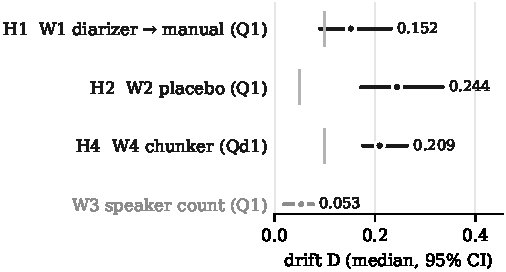
\includegraphics[width=\columnwidth]{figs/drift.pdf}
\caption{Drift of the primary query per workload on held-out units: median and 95\% BCa interval. Black: confirmatory
tests; gray: exploratory. Short vertical ticks mark each hypothesis' preregistered threshold $T$.}
\label{fig:drift}
\end{figure}
\begin{figure}[t]
\centering
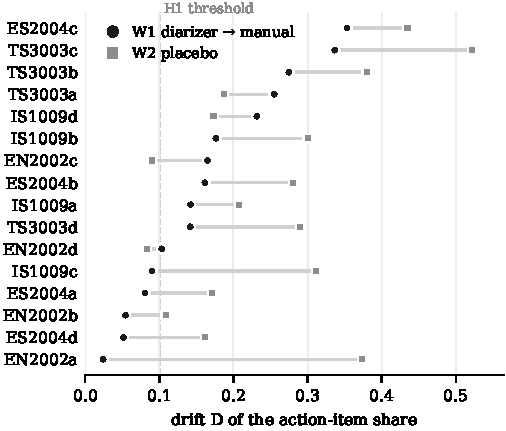
\includegraphics[width=\columnwidth]{figs/per_unit.pdf}
\caption{Per-meeting drift of the action-item share on the 16 held-out meetings, sorted by W1 drift. Dashed: the H1
threshold $T$.}
\label{fig:perunit}
\end{figure}

% ---------------------------------------------------------------- 5. RQ2 (1.25 pp; Fig. 3)
\section{RQ2: Granularity or Boundaries?}\label{sec:rq2}
\textbf{H2} (supported). The placebo changes the action-item share by \nHtwomed{} (\nHtwolo--\nHtwohi), although it
preserves the words, the number of segments and their lengths. Per meeting, the placebo drift exceeds the W1 drift
by a median \nPlaceboGapmed{} (\nPlaceboGaplo--\nPlaceboGaphi; larger in \nPlaceboGaplarger{} of 16 meetings); with
the 0.5B model the difference is not significant on these 16 meetings (\nPlaceboGapMtwolo--\nPlaceboGapMtwohi) but is
on \nScaleN{} further meetings (Sec.~\ref{sec:dir}). This does not identify the
cause of W1's drift, but it shows that drift of this size does not require diarization errors: an arbitrary move of
boundaries, with words, segment count and sizes held fixed, produces at least as much.
\paragraph*{Where the flips are} Aggregates hide how much changes underneath. Under W1, \nFlipWoneactionitem\% of words
change their action-item label (question \nFlipWonequestion\%, topic \nFlipWonetopic\%); under the placebo,
\nFlipWtwoactionitem\%. Flips in the two directions largely cancel, so the
net change of a share is much smaller than the flip rate; the drift $D$ is that remainder relative to the old share. Flips concentrate where a word's segment changes length: in
W1, a word whose new segment is within 0.8--1.25$\times$ the length of its old one flips \nFlipWonesame\% of the time,
against \nFlipWonehalf\% when the segment shrinks below half and \nFlipWonedouble\% when it more than doubles. The
placebo keeps the length distribution but not each word's segment length; even words whose segment length is nearly
unchanged flip \nFlipWtwosame\% of the time, because the words around them change.
\paragraph*{Granularity amplifies} Boundaries are not the only factor. Merging $k$ consecutive same-speaker manual
segments keeps every boundary of the coarser segmentation at an original boundary but makes segments $k$ times longer.
Drift grows steeply with $k$ (Fig.~\ref{fig:gran}): \nEsixktwoQonemed{} (\nEsixktwoQonelo--\nEsixktwoQonehi) at $k=2$,
\nEsixkfourQonemed{} at $k=4$, and \nEsixkeightQonemed{} (\nEsixkeightQonelo--\nEsixkeightQonehi) at $k=8$. Granularity
is thus a second lever beside boundary placement; W1, which refines the segmentation, drifts less than the placebo.
\begin{figure}[t]
\centering
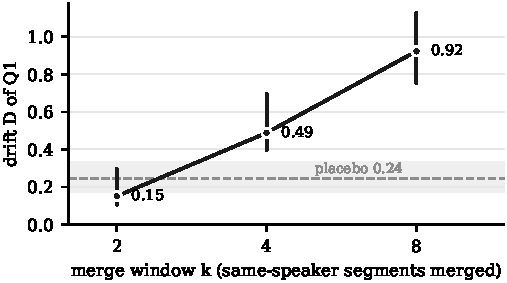
\includegraphics[width=\columnwidth]{figs/granularity.pdf}
\caption{Granularity dose--response on held-out meetings: drift of the action-item share when $k$ consecutive
same-speaker manual segments are merged (median and 95\% interval). Dashed line and gray band: the placebo (median
and interval), which keeps segment sizes and only moves boundaries; it is a reference, not a point on the $k$ axis.}
\label{fig:gran}
\end{figure}

% ---------------------------------------------------------------- 6. RQ3 (1.0 pp; Tab. 2)
\section{RQ3: Pipeline Revisions and Documents}\label{sec:rq3}
\textbf{H4} (supported). Switching the chunker changes the dated share of Wikipedia text by \nHfourmed{}
(\nHfourlo--\nHfourhi; \nHfourvalid{} of \nHfourunits{} articles, \nHfourguard{} excluded by the 0.02 guard); entity
sums change by \nWikiQdtwomed{} and the topic distribution by a total variation of \nWikiQdthreemed.
\textbf{Window size} (post-hoc). A routine setting, the window of the same fixed chunker, also moves the answer:
from 120 to 150 words the dated share changes by \nChunkonefivezeromed{} (absolute \nChunkonefivezeroabs{} points,
rising in \nChunkonefivezeroup{} of 200 articles), and from
120 to 100 words by \nChunkonezerozeromed{} (absolute \nChunkonezerozeroabs, rising in \nChunkonezerozeroup). Many
articles have only a few chunks, so per-article drift takes values such as $1/6$ and $1/4$ and the medians and
interval ends fall on them; the means are larger (\nChunkonefivezeromean{} and \nChunkonezerozeromean, absolute
\nChunkonefivezeroabsmean{} and \nChunkonezerozeroabsmean{} points), and the dated share changes at all in
\nChunkonefivezerochanged{} and \nChunkonezerozerochanged{} of 200 articles.
\textbf{W3} (exploratory). A diarizer configuration change (estimated vs known speaker count) changes the action-item
share by only \nWthreeQonemed{} (\nWthreeQonelo--\nWthreeQonehi); it changes a third of the segments
(Table~\ref{tab:workloads}), against almost all of them under W1.
\paragraph*{A second model and other queries} With Qwen2.5-0.5B the primary effects reappear (Table~\ref{tab:all}): W1
\nWoneQoneMtwomed{} (\nWoneQoneMtwolo--\nWoneQoneMtwohi), placebo \nWtwoQoneMtwomed{} (\nWtwoQoneMtwolo--\nWtwoQoneMtwohi),
chunker \nWikiQdoneMtwomed{} (\nWikiQdoneMtwolo--\nWikiQdoneMtwohi). With this model the placebo is not clearly larger
than W1 on these 16 meetings (paired difference \nPlaceboGapMtwomed, interval \nPlaceboGapMtwolo--\nPlaceboGapMtwohi);
on the \nScaleN{} scale meetings it is (Sec.~\ref{sec:dir}), and the placebo's median drift exceeds W1's for all five
scorers (Table~\ref{tab:models}). Across queries, shares of binary and label columns move
most; entity sums and topic distributions move less on meetings but strongly on documents. The 0.5B model almost
never answers ``cost'', so that query has no valid unit for it.
\paragraph*{Larger models and another family (post-hoc)} Table~\ref{tab:models} adds Qwen2.5-3B and -7B and Microsoft's
Phi-3.5-mini (3.8B), each in fp32 and each with identical labels under two batch budgets before use (3B and Phi on the
TITAN Xp cards, split over two; 7B on one NVIDIA A100 80\,GB; a bf16 run of
7B failed this check and was discarded). These three were run on W1, W2 and W4 only; every scorer's relative drift is
positive on each, though for 3B and 7B the absolute W1 change of the action-item share is within a point of zero.
All scorers are weak judges of these columns (Sec.~\ref{sec:dir}), so drift is measured on labels of limited validity;
the two that agree best with the human labels still drift: Phi-3.5-mini (question
F1 \nGoldQumanualfoneMphi) changes the action-item share by \nWoneQoneMphimed{} under W1, \nWtwoQoneMphimed{} under
the placebo (more than under W1 by \nPlaceboGapMphimed, \nPlaceboGapMphilo--\nPlaceboGapMphihi) and the dated share
by \nWikiQdoneMphimed{} under the chunker change; Qwen2.5-7B (question F1 \nGoldQumanualfoneMseven) changes the
question share by \nWoneQtwoMsevenmed{} (\nWoneQtwoMsevenlo--\nWoneQtwoMsevenhi) under W1 and \nWtwoQtwoMsevenmed{}
(\nWtwoQtwoMsevenlo--\nWtwoQtwoMsevenhi) under the placebo, and the dated share by \nWikiQdoneMsevenmed{}, the smallest
chunker drift of the five scorers. Relative drift must be read with the base share: 3B and 7B label far less speech
as action items (median old share \nSgWoneQoneMthreeold\% and \nSgWoneQoneMsevenold\% against \nSgWoneQoneold\% for
1.5B), so their relative drift is larger while their absolute changes are smaller; for 7B only
\nWoneQoneMsevenvalid{} of 16 meetings pass the guard on this query, and its absolute W1 change is \nSgWoneQoneMsevenabs{}
points (\nSgWoneQoneMsevenabslo{} to \nSgWoneQoneMsevenabshi). The absolute
columns therefore matter as much as $D$: a consumer who compares answers across versions sees the relative change, one
who reads levels sees the absolute one.
\paragraph*{Drift is not a matter of near-ties (post-hoc)} A scorer could drift only because many of its labels are
coin flips that any change of input tips over. We recompute the question and action-item shares over segments whose
answer logit leads the runner-up by at least \nConfMargin{} (about 88\% confidence for a yes/no answer) on both sides.
For the three larger scorers most words pass (\nConfWoneQtwoSevenkept\% for 7B, \nConfWoneQtwoThreekept\% for 3B and
\nConfWoneQonePhikept\% for Phi on W1), and drift does not shrink: W1 question drift is \nConfWoneQtwoSevenmed{}
(\nConfWoneQtwoSevenlo--\nConfWoneQtwoSevenhi) for 7B and \nConfWoneQtwoThreemed{} for 3B, placebo action-item drift
\nConfWtwoQonePhimed{} (\nConfWtwoQonePhilo--\nConfWtwoQonePhihi) for Phi. For action items under W1 the guard leaves
only \nConfWoneQoneSevenn{} (7B) and \nConfWoneQoneThreen{} (3B) meetings and the intervals reach
\nConfWoneQoneSevenhi{} and \nConfWoneQoneThreehi, so those cells are uninformative. The two small models are rarely
that confident (\nConfWoneQtwokept\% of words for 1.5B), so this test says little about them.
\begin{table*}[t]
\centering\footnotesize
\caption{Post-hoc: every scorer on held-out data. Base share: median old action-item share. $D$: median relative
drift of the primary query (W1, W2: action items; W4: dated text). $|\Delta|$: median absolute change in percentage
points, regardless of direction. Question F1: word-level agreement with human dialogue-act labels on manual segments.}
\label{tab:models}
% generated by paper/figs/models.py
\begin{tabular}{@{}lrrrrrrrr@{}}
\toprule
& base & \multicolumn{2}{c}{W1 diarizer$\to$manual} & \multicolumn{2}{c}{W2 placebo} & \multicolumn{2}{c}{W4 chunker} & question \\
\cmidrule(lr){3-4}\cmidrule(lr){5-6}\cmidrule(lr){7-8}
scorer & share \% & $D$ & $|\Delta|$ pts & $D$ & $|\Delta|$ pts & $D$ & $|\Delta|$ pts & F1 \\
\midrule
Qwen2.5-0.5B & 21.9 & 0.13 & 2.8 & 0.16 & 3.4 & 0.33 & 16.0 & 0.04 \\
Qwen2.5-1.5B (primary) & 28.8 & 0.15 & 4.4 & 0.24 & 6.0 & 0.21 & 11.9 & 0.14 \\
Qwen2.5-3B & 3.2 & 0.29 & 1.6 & 0.78 & 2.0 & 0.27 & 6.5 & 0.19 \\
Qwen2.5-7B & 1.9 & 0.20 & 0.5 & 0.73 & 1.0 & 0.10 & 5.5 & 0.30 \\
Phi-3.5-mini (3.8B) & 15.8 & 0.17 & 2.8 & 0.35 & 5.7 & 0.33 & 9.8 & 0.24 \\
\bottomrule
\end{tabular}

\end{table*}
\begin{table*}[t]
\centering\footnotesize
\caption{Median relative drift $D$ on held-out units for every query and workload, for the 0.5B, 1.5B and 3B models
(exploratory, except the primary queries of W1, W2 and W4 with the 1.5B model; the 3B model is post-hoc and was not
run on W3; 7B and Phi are in Table~\ref{tab:models}). ``--'': no unit passes the 0.02
guard. Intervals and absolute changes are in the released tables.}
\label{tab:all}
% generated by paper/figs/drift_all.py
\begin{tabular}{@{}lcccccccc@{}}
\toprule
& \multicolumn{3}{c}{W1 diarizer $\to$ manual} & \multicolumn{3}{c}{W2 placebo} & \multicolumn{2}{c}{W3 speaker count} \\
\cmidrule(lr){2-4}\cmidrule(lr){5-7}\cmidrule(lr){8-9}
query & 1.5B & 0.5B & 3B & 1.5B & 0.5B & 3B & 1.5B & 0.5B \\
\midrule
action item & 0.15 & 0.13 & 0.29 & 0.24 & 0.16 & 0.78 & 0.05 & 0.03 \\
question & 0.10 & 0.11 & 0.31 & 0.26 & 0.42 & 0.29 & 0.03 & 0.04 \\
neg.\ sentiment & 0.18 & 0.08 & 0.11 & 0.18 & 0.14 & 0.37 & 0.05 & 0.03 \\
topic = cost & 0.13 & -- & 0.27 & 0.35 & -- & 0.24 & 0.05 & -- \\
entity sum & 0.07 & 0.05 & 0.04 & 0.07 & 0.27 & 0.20 & 0.01 & 0.02 \\
topic distance & 0.06 & 0.02 & 0.06 & 0.08 & 0.03 & 0.05 & 0.01 & 0.01 \\
\midrule
\multicolumn{9}{@{}l}{\textit{W4, Wikipedia test (chunker change)}} \\
dated text & \multicolumn{8}{l}{1.5B 0.21 \quad 0.5B 0.33 \quad 3B 0.27} \\
entity sum & \multicolumn{8}{l}{1.5B 0.42 \quad 0.5B 0.55 \quad 3B 0.35} \\
topic distance & \multicolumn{8}{l}{1.5B 0.11 \quad 0.5B 0.19 \quad 3B 0.10} \\
\bottomrule
\end{tabular}

\end{table*}

% ---------------------------------------------------------------- 6b. Direction and correctness (post-hoc, D5)
\section{Direction and Correctness}\label{sec:dir}
The analyses in this section were added after the confirmatory analysis, following an internal review; they are
post-hoc and exploratory (logged as a deviation before they were run).
\paragraph*{Drift has a direction when the re-segmentation is systematic} Relative drift $D$ is unsigned. Signed,
absolute changes separate erratic from systematic movement. Merging segments raises the yes-share of predicates that
are satisfied by \emph{any} part of a segment: at $k=8$ the action-item share rises by a median
\nSgEsixkeightQoneabs{} percentage points (in \nSgEsixkeightQoneup{} of 16 meetings) and the question share by
\nSgEsixkeightQtwoabs{} (\nSgEsixkeightQtwoup{} of 16), while the share of negative sentiment, a judgment about the
whole segment, falls by \nSgEsixkeightQthreeabs{} (rising in only \nSgEsixkeightQthreeup{} of 16) (merges were scored
with the primary model only). The placebo, which cuts utterances at arbitrary words, changes the question share by
\nSgWtwoQtwoabs{} points with the primary model, and the question share falls for four of the five scorers (it rises
in \nSgWtwoQtwoup, \nSgWtwoQtwoMtwoup, \nSgWtwoQtwoMthreeup{} and \nSgWtwoQtwoMphiup{} of 16 meetings for the 1.5B,
0.5B, 3B and Phi models): a question split across two segments is often recognized in neither. Qwen2.5-7B is the
exception: its question share rises by \nSgWtwoQtwoMsevenabs{} points (\nSgWtwoQtwoMsevenabslo{} to
\nSgWtwoQtwoMsevenabshi; in \nSgWtwoQtwoMsevenup{} of 16), as if it recognized a question in both halves. For action
items the direction depends on the model: the share rises in \nSgWtwoQoneup{} of 16 meetings for 1.5B,
\nSgWtwoQoneMtwoup{} for 0.5B, \nSgWtwoQoneMthreeup{} for 3B, \nSgWtwoQoneMsevenup{} for 7B and \nSgWtwoQoneMphiup{}
for Phi. Replacing diarizer turns by manual segments (W1) has no clear direction on the 16 held-out meetings
(\nSgWoneQoneabs{} points, interval \nSgWoneQoneabslo{} to \nSgWoneQoneabshi; rising in \nSgWoneQoneup{} of 16; see the
scale run below), and
paragraph chunking raises the dated share of articles by \nSgWikiQdoneabs{} points (rising in \nSgWikiQdoneup{} of
200). Segmentation can therefore bias LLM-derived aggregates: with the primary model, coarsening raised predicates satisfied by
any part of a segment, while the direction under arbitrary cuts depends on the predicate and the scorer.
\paragraph*{Drift changes agreement with human labels} AMI's manual dialogue acts give a human reference for two
columns: questions (elicit acts) and, as a proxy for action items, suggestions; both type sets were fixed in an earlier
pilot. Table~\ref{tab:gold} compares each segmentation's word-weighted share with the human share. The scorer
over-predicts both predicates under every segmentation (its notion of a question is broader than an elicit act; the
human question share is \nGoldQushare\%). Across the segmentations a pipeline would produce (manual, diarizer turns,
estimated speaker count) the question-share error varies modestly, from \nGoldQumanualabserr{} to
\nGoldQuwoneoldabserr{} points; across coarser segmentations it grows to \nGoldQumergeeightabserr{} points; across
scorers on the same manual segments it ranges from \nGoldQumanualabserrMphi{} (Phi-3.5-mini) to
\nGoldQumanualabserr{} (1.5B).
Lower share error is not better segmentation: the placebo looks closest only because it pushes shares down. Word-level
F1, which does not reward such compensation, is \nGoldQumanualfone{} for manual segments and \nGoldQuwoneoldfone{} for
diarizer turns on questions with the primary model, and \nGoldQumanualfoneMthree{} under each of the three
segmentations scored with the 3B model. The accuracy of an LLM-derived aggregate therefore depends on both the scorer and the segmentation, and
neither can be reported without the other.
\paragraph*{Scale} To test whether the held-out results generalize beyond 16 meetings, we diarized and scored the
\nScaleN{} remaining AMI meetings (all except dev, eval and one whose audio could not be downloaded) with the second
model, on a second server whose labels matched the first on all 1,000 rescored cells. These meetings include AMI's
training split, on which pyannote's segmentation model was trained, so its turns may be better there than on unseen
audio; the placebo does not involve pyannote. Drift is stable as the sample
grows (Fig.~\ref{fig:scale}): with all \nScaleN{} meetings, W1 changes the action-item share by \nScaleWoneQonemed{}
(\nScaleWoneQonelo--\nScaleWoneQonehi) and the placebo by \nScaleWtwoQonemed{} (\nScaleWtwoQonelo--\nScaleWtwoQonehi),
and the interval of W1 narrows from \nScaleWoneQonesixteenwidth{} for the first 16 scale meetings to
\nScaleWoneQonefullwidth. The
placebo now drifts more than W1 also for this model (paired difference \nScaleGapmed, \nScaleGaplo--\nScaleGaphi;
larger in \nScaleGaplarger{} of \nScaleN{} meetings), which the 16 held-out meetings could not resolve. The
held-out directions for this model also hold at scale: the placebo lowers the question share in
\nScaleWtwoQtwodown{} of \nScaleN{} meetings and raises the action-item share in \nScaleWtwoQoneup. Materializing
one five-column view of the \nScaleN{} meetings takes \nScaleCallsManual{} calls, about \nScaleMinManual{} minutes on
one card for the 0.5B model; the number of calls grows linearly with the corpus, and so does the cost of every full
recomputation that non-invariance forces.
\paragraph*{Scale with the primary model (post-hoc)} We repeated the scale run with the 1.5B model on the same server,
after checking that it reproduces the first server's held-out labels exactly (\nXhostPmism{} of \nXhostPN{} cells
differ). Over the \nScalePN{} meetings, W1 changes the action-item share by \nScalePWoneQonemed{}
(\nScalePWoneQonelo--\nScalePWoneQonehi), above the held-out estimate of \nHonemed, and the question share by
\nScalePWoneQtwomed; the placebo changes them by \nScalePWtwoQonemed{} and \nScalePWtwoQtwomed{} and again exceeds W1
(paired difference \nScalePGapmed, \nScalePGaplo--\nScalePGaphi). The directions seen on the held-out meetings become
clear: manual segments lower the action-item share relative to diarizer turns by \nScalePWoneQoneabs{} points
(rising in only \nScalePWoneQoneup{} of \nScalePN{} meetings, where the held-out interval still included zero), and the
placebo lowers both shares (rising in \nScalePWtwoQoneup{} and \nScalePWtwoQtwoup{}). These meetings are a
different population (they include pyannote's training data), so the run supports the direction and existence of
drift, not a correction of the held-out estimates.
\begin{figure}[t]
\centering
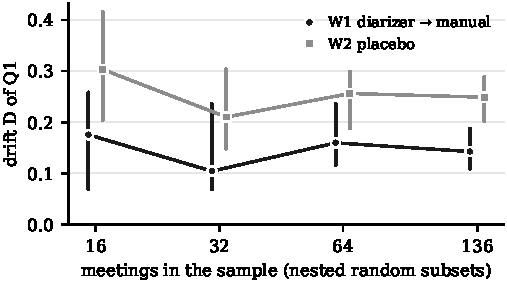
\includegraphics[width=\columnwidth]{figs/scale.pdf}
\caption{Post-hoc scale check with the second model: drift of the action-item share on nested random subsets of the
\nScaleN{} AMI meetings outside the development and held-out sets (median and 95\% interval).}
\label{fig:scale}
\end{figure}
\begin{table}[t]
\centering\footnotesize
\caption{Post-hoc: word-weighted shares under each segmentation of the held-out meetings versus human dialogue-act
labels (median over 16 meetings, \%; primary model). $|$err$|$: absolute difference to the human share. F1: word-level
agreement with the human labels.}
\label{tab:gold}
\setlength{\tabcolsep}{4pt}
% generated by paper/figs/gold.py
\begin{tabular}{@{}lrrrrrr@{}}
\toprule
& \multicolumn{3}{c}{question} & \multicolumn{3}{c}{action item (proxy)} \\
\cmidrule(lr){2-4}\cmidrule(lr){5-7}
segmentation & share & $|$err$|$ & F1 & share & $|$err$|$ & F1 \\
\midrule
human labels & 4.4 & & & 10.3 & & \\
\midrule
manual & 48.4 & 42.3 & 0.14 & 27.2 & 15.0 & 0.24 \\
diarizer (W1 old) & 50.8 & 47.6 & 0.10 & 28.7 & 19.8 & 0.25 \\
diarizer, est.\ count & 50.5 & 45.4 & 0.11 & 27.4 & 18.3 & 0.25 \\
placebo & 33.5 & 28.2 & 0.14 & 20.7 & 11.7 & 0.19 \\
merge $k=2$ & 56.6 & 51.4 & 0.12 & 30.8 & 20.0 & 0.25 \\
merge $k=4$ & 64.5 & 58.8 & 0.11 & 41.0 & 30.6 & 0.27 \\
merge $k=8$ & 77.4 & 73.8 & 0.09 & 61.3 & 46.0 & 0.23 \\
\bottomrule
\end{tabular}

\end{table}

% ---------------------------------------------------------------- 6c. Calibration, a candidate fix, structure (post-hoc, D6)
\section{How Large, and Can Context Fix It?}\label{sec:calib}
This section is also post-hoc (a second logged deviation, after a second internal review).
\paragraph*{A scale for drift} To read a drift of 0.15, we measure the same statistic for two changes that pipelines
already treat as versioned, on the \emph{fixed} manual segmentation of the held-out meetings. Four rewordings of each
column question, with the same answer sets and scoring, change the action-item share by a median \nCalParaDQonemed,
\nCalParaQonemed, \nCalParaBQonemed{} and \nCalParaCQonemed{}, and the question share by \nCalParaBQtwomed{} to
\nCalParaCQtwomed{} (absolute \nCalParaBQtwoabs{} to \nCalParaCQtwoabs{} points: what counts as a question shifts with
its wording). The first rewording with the 0.5B scorer changes the action-item share by \nCalParaHalfQonemed{}
against a W1 drift of \nWoneQoneMtwomed{} for that model. Replacing the 1.5B scorer by the 0.5B one changes the action-item share by
\nCalSwapHalfQonemed, and by Phi-3.5-mini or 3B by \nCalSwapPhiQonemed{} and \nCalSwapThreeQonemed{} (all on the same
cards; the 7B model ran on other hardware and is not compared here). W1 drift (\nHonemed{} for action items,
\nWoneQtwomed{} for questions) is thus just below the mildest rewording for action items, and about a fifth of the
mildest for questions; the placebo's action-item drift (\nHtwomed) lies within the range of the rewordings, and both
segmentation drifts are smaller than any of the three model swaps. Segmentation is a smaller lever than the prompt, but for action items of the
same order as its mildest rewordings. Prompts and models are routinely recorded with an LLM-derived
result; the segmentation usually is not.
\paragraph*{Context padding is not a fix} A natural remedy is to let the scorer see the neighbors of each segment:
we show the two preceding and two following segments as context and label only the target, as DocETL's gather
operator does for split documents~\cite{docetl}. This costs
\nCtxRatio$\times$ the input tokens (\nCtxTokCtx{} instead of \nCtxTokPlain{} per call). It lowers W1 drift (action
items \nWoneQoneCtxmed{} instead of \nHonemed; questions \nWoneQtwoCtxmed{} instead of \nWoneQtwomed) and placebo drift
for questions (\nWtwoQtwoCtxmed{} instead of \nWtwoQtwomed), but raises placebo drift for action items to
\nWtwoQoneCtxmed{}, and it reduces agreement with the human labels (question F1 \nGoldQumanualfoneCtx{} instead of
\nGoldQumanualfone{} on manual segments) because the model then labels more of the speech as questions. Context
changes what the view measures as much as it stabilizes it; a segmentation-robust view needs more than a wider prompt.
\paragraph*{Structure, formally} Structural reuse would be sound for predicates that compose over segments.
\begin{proposition}\label{prop:mono}
Let $f$ be a binary column that is monotone under concatenation: $f(st) \ge \max(f(s), f(t))$ with yes $>$ no. If
$S'$ coarsens $S$ (every segment of $S'$ is a concatenation of consecutive segments of $S$), then
$Q_{f,\mathrm{yes}}(S') \ge Q_{f,\mathrm{yes}}(S)$.
\end{proposition}
\begin{proof}
A word labeled yes under $S$ lies in a segment $s$ with $f(s)=$ yes; its segment under $S'$ contains $s$, so it is
labeled yes as well. Word weights do not change.
\end{proof}
Action items and questions are intended to be such ``any part'' predicates, and merging indeed raises their shares
(Sec.~\ref{sec:dir}). But the scorer violates monotonicity often: among merged segments with at least two parts,
\nMonoktwoAcloss\% (at $k=2$) to \nMonokeightAcloss\% (at $k=8$) are labeled ``no'' although one of their parts was
labeled ``yes'' (questions: \nMonoktwoQuloss\% to \nMonokeightQuloss\%). The rules of Sec.~\ref{sec:rq4} therefore
cannot be trusted without verification, and reusing the overlapping old value is no better: it is right for only
\nAnchorAccactionitem\% of changed action-item cells, \nAnchorAccquestion\% of question cells and
\nAnchorAcctopic\% of topic cells.

% ---------------------------------------------------------------- 7. RQ4 (1.75 pp; Tab. 3, Fig. 4)
\section{RQ4: Consequences for View Maintenance}\label{sec:rq4}
When a segmenter is revised, a view must be brought up to date. Recomputing every changed row is always correct; the
question is how much of that cost can be avoided without returning wrong cells. We replay five policies on the cached
outputs of W1 (\nEWonecells{} changed cells over 16 held-out meetings and five columns), so every policy's LLM calls
and its true cell error are known exactly.
\paragraph*{Policies}
\emph{Full} recomputes every changed cell. \emph{Content hash} reuses a value only when the new segment's text equals
an old segment's text; this is exact. \emph{Anchor + audit} transfers the stable-row view of prior work~\cite{sivm,semreuse}, which was not designed for
re-segmentation, to this setting:
it gives each new cell the value of its most-overlapping old segment (its anchor) as a provisional value and certifies
it per column with an exact hypergeometric audit. \emph{Rules/anchor + audit} proposes values from structural
rules where they apply (e.g., a segment whose parts are all ``no'' for a monotone predicate is ``no''; an entity count
of a segment that is the exact union of old segments is their sum) and from anchors elsewhere, and audits each
provenance stratum. The audit samples a stratum with doubling sample sizes and certifies it when the $(1-\alpha)$ upper
bound on its number of wrong provisional values is at most $\epsilon N$; an uncertifiable stratum is recomputed; the
family error $\delta=0.05$ is split over strata (union bound). A further variant splits strata by the scorer's
confidence on the old cells.
\begin{table*}[t]
\centering\footnotesize
\caption{View maintenance on held-out meetings: LLM calls as a share of full recomputation, with the 95\% interval of
a meeting bootstrap in which the whole policy is re-run in each resample, and the true cell error in percent; means
of 100 trials, family error $\delta=0.05$. Content hashing does not depend on $\epsilon$ and has no error.}
\label{tab:maint}
% generated by paper/figs/maintenance.py
\begin{tabular}{@{}lrrrrrrrr@{}}
\toprule
policy & \multicolumn{2}{c}{$\epsilon=0.02$} & \multicolumn{2}{c}{$\epsilon=0.05$} & \multicolumn{2}{c}{$\epsilon=0.10$} & \multicolumn{2}{c}{$\epsilon=0.15$} \\
\cmidrule(lr){2-3}\cmidrule(lr){4-5}\cmidrule(lr){6-7}\cmidrule(lr){8-9}
& calls & err.\% & calls & err.\% & calls & err.\% & calls & err.\% \\
\midrule
\multicolumn{9}{@{}l}{\textit{W1: 36,385 changed cells}} \\
content hash (exact) & 0.742 [0.72, 0.76] & 0.00 & 0.742 [0.72, 0.76] & 0.00 & 0.742 [0.72, 0.76] & 0.00 & 0.742 [0.72, 0.76] & 0.00 \\
anchor + audit & 0.742 [0.72, 0.76] & 0.00 & 0.742 [0.72, 0.76] & 0.00 & 0.742 [0.72, 0.76] & 0.00 & 0.742 [0.72, 0.76] & 0.00 \\
rules/anchor + audit & 0.742 [0.72, 0.76] & 0.00 & 0.734 [0.71, 0.76] & 0.03 & 0.639 [0.61, 0.68] & 0.57 & 0.567 [0.54, 0.61] & 1.22 \\
\quad + confidence strata & 0.738 [0.72, 0.76] & 0.00 & 0.724 [0.70, 0.74] & 0.02 & 0.671 [0.63, 0.71] & 0.33 & 0.565 [0.53, 0.61] & 1.24 \\
\midrule
\multicolumn{9}{@{}l}{\textit{W3: 10,970 changed cells}} \\
content hash (exact) & 0.526 [0.48, 0.56] & 0.00 & 0.526 [0.48, 0.56] & 0.00 & 0.526 [0.48, 0.56] & 0.00 & 0.526 [0.48, 0.56] & 0.00 \\
anchor + audit & 0.526 [0.48, 0.56] & 0.00 & 0.526 [0.48, 0.56] & 0.00 & 0.526 [0.48, 0.56] & 0.00 & 0.509 [0.44, 0.54] & 0.22 \\
rules/anchor + audit & 0.526 [0.48, 0.56] & 0.00 & 0.526 [0.48, 0.56] & 0.00 & 0.476 [0.44, 0.51] & 0.28 & 0.431 [0.39, 0.46] & 0.56 \\
\quad + confidence strata & 0.526 [0.48, 0.56] & 0.00 & 0.523 [0.48, 0.55] & 0.01 & 0.494 [0.45, 0.53] & 0.15 & 0.454 [0.41, 0.48] & 0.38 \\
\bottomrule
\end{tabular}

\end{table*}
\paragraph*{Results (Table~\ref{tab:maint})}
Content hashing is exact and needs \nEWonehashshare{} of the calls: \nEWonehashpct\% of changed cells keep an identical
text, because only their times moved. Under W1, anchor reuse with an audit saves nothing beyond hashing at any
$\epsilon$: the anchors are wrong too often for any stratum to certify, so every non-identical cell is recomputed.
Under the smaller W3 revision it certifies a little at $\epsilon=0.15$ (\nEWthreeanchorcertepsonefiveshare{} of calls
against \nEWthreehashshare{} for hashing). This is the practical meaning of non-invariance for stable-row maintenance. Structural rules help only modestly: on the \nEWonerulecells{} cells where a rule fires,
\nEWonerulesmajority{} of the \nEWonerulesn{} rules are exactly as accurate as predicting the majority class
(Cohen's $\kappa=0$); only the entity-sum rule carries information ($\kappa=\nEWonesumunionkappa$). With the audit, rules plus
anchors need
\nEWoneechobaseepsonezeroshare{} of the calls at $\epsilon=0.10$ (cell error \nEWoneechobaseepsonezeroerr) and
\nEWoneechobaseepsonefiveshare{} at $\epsilon=0.15$. The share of trials in which any certified stratum's true error
exceeded $\epsilon$ was \nEWoneechobaseepsonezeroviol{} at $\epsilon=0.10$ and \nEWoneechobaseepsonefiveviol{} at
$\epsilon=0.15$, within $\delta=0.05$.
\paragraph*{Why the audit saves so little (post-hoc)} We corrupt the provisional values of the \nPowerStrata{} largest
strata to a known true error from $\epsilon-0.05$ to $\epsilon+0.05$ and run the audit 100 times at each level. The audit is exact by construction, and the simulation agrees: a stratum
whose actual error exceeds $\epsilon$ is certified at an observed rate of at most \nPowerViolMax{}, against a
per-stratum allowance of \nPowerAlpha{} (with so few events this is a consistency check, not a further proof). It is also expensive. With the family
error split over all strata, each stratum must be audited at a very small risk, and even when every provisional value
is correct the audit recomputes \nPowerSampZero\% of the stratum at $\epsilon=0.05$; at two points below the tolerance
it recomputes \nPowerSampBelowfive--\nPowerSampBelowonefive\%, and at the tolerance essentially all of it. Certified
reuse therefore pays off only for large strata whose provisional values are far more accurate than $\epsilon$, which
re-segmentation does not produce. The union bound is not the cause: pooling all \nPoolWoneanchored{} anchored cells
of W1 into one stratum audited at the full $\delta$ (a weaker guarantee, on the overall error only) certifies in none of
100 trials at any $\epsilon$ up to 0.15, because the old row's value is wrong for \nPoolWoneanchorerr\% of these cells
(\nPoolWthreeanchorerr\% under W3); no audit can certify reuse at that error rate.
\paragraph*{Cost} A recomputed cell is one scorer call on a segment of \nEWonetok{} tokens on average. At the measured
rate of \nThrBig{} calls per second, recomputing all changed cells of W1 takes \nMaintMinFull{} GPU-minutes on one
card; content hashing \nMaintMinHash{}, and rules with the audit at $\epsilon=0.10$ \nMaintMinRules{} (mean over
trials). The audit itself is CPU work and cheap: replaying all policies, tolerances, trials and bootstrap resamples
(\nEWonepolicyruns{} complete maintenance runs plus the validity test) takes \nEWonewall{} minutes, at most
\nEWonesecperrun{} seconds per run. These are small numbers because our views are small; the shares in Table~\ref{tab:maint} are
what transfers to larger deployments, where calls are billed per token or bounded by GPU time.
Under W3, where only a third of the segments change, content hashing already avoids about half of the calls
(\nEWthreehashshare{} remain) and the audit reduces them to \nEWthreeechobaseepsonezeroshare{} at $\epsilon=0.10$ (Table~\ref{tab:maint}).
The smaller the revision, the more of the view survives by content alone.

% ---------------------------------------------------------------- 9. Related work (0.75 pp)
\section{Related Work}
\paragraph*{Semantic operators and LLM-derived data} Generating structured views of unstructured data with LLMs is an
established data-management task: Evaporate builds queryable tables from heterogeneous document collections and
trades extraction quality against LLM cost~\cite{evaporate}. Semantic data systems execute LLM calls as query
operators: LOTUS defines declarative semantic operators with accuracy guarantees~\cite{lotus}, Palimpzest optimizes
AI analytics for cost, runtime and quality~\cite{palimpzest}, DocETL rewrites document-processing pipelines with an
agent~\cite{docetl}, ZenDB answers SQL over templated documents using their structure~\cite{zendb}, and Stretto is an
execution engine for such systems~\cite{stretto}. All of them operate on rows that an upstream step has already
produced (tuples, documents, chunks) or derive the units from document structure~\cite{zendb}; we are not aware
of one that measures how query answers depend on that choice of units. Recent work maintains their results under change: SemReuse certifies the reuse of cached
natural-language views for new semantic predicates~\cite{semreuse}; sIVM certifies the maintenance of LLM-computed
cells under prompt edits~\cite{sivm}; and maintaining an evolving semantic substrate can cost in proportion to the
change rather than the corpus~\cite{costchange}. All of them key results by a stable row or document identity. We study
the change they assume away: the rows themselves move while the content stays fixed, and we show that this alone
changes the answers.
\paragraph*{View maintenance, provenance and evolving text} Materialized-view maintenance avoids recomputation by
detecting updates that cannot affect a view and re-evaluating the rest differentially~\cite{blakeley86}; it is now
part of industrial data-engineering pipelines~\cite{enzyme}. Its correctness rests on the view being a function of
the base data. For LLM-derived views this holds only once the segmentation is fixed, so we treat the segmenter as part
of the view definition (Sec.~\ref{sec:model}) and measure what maintenance costs when it changes
(Sec.~\ref{sec:rq4}). Our structural rules and anchors are a form of where-provenance~\cite{whywhere}: they map a
new segment to the old segments its words came from. Cyclex recycles information-extraction results across snapshots
of evolving text~\cite{cyclex}, for extractors whose outputs are tied to text regions. LLM extractors read a whole
segment, so the segment boundary is part of the input; Propositions~\ref{prop:trivial} and~\ref{prop:mono} make this
precise.
\paragraph*{Sensitivity of LLMs} NLP work shows that LLM outputs change under semantically equivalent prompt
formats~\cite{sclar}. We hold the prompt fixed and change only how the data are cut, a decision made by a data
pipeline, and measure the effect on aggregate query answers rather than on single outputs.
\paragraph*{Segmenters} Speaker diarization~\cite{pyannote} and document chunking decide the rows of segment-keyed
views; they are evaluated by their own error metrics, not by the stability of downstream analytical answers. In
meeting processing, dialog-act classification is known to degrade with automatic segmentation and recognized words
rather than human ones~\cite{angdialog}; there the words change too and the target is per-segment accuracy, while we
hold the words fixed and measure aggregate query answers. In
retrieval-augmented generation, chunking is tuned for answer quality: a systematic study finds that overlap brings no
benefit and that sentence chunking is the most cost-effective method~\cite{chunkqa}. We ask a different question:
not which chunking answers best, but how much an aggregate changes when the chunking changes.
\paragraph*{Unit-of-aggregation effects} That aggregates depend on the units over which data are grouped is known in
spatial statistics as the modifiable areal unit problem~\cite{maup}. Our setting differs in where the dependence
arises: the measurement itself (the LLM's label of a unit) changes with the unit, not only the aggregation, and the
direction follows the predicate (Sec.~\ref{sec:dir}).

% ---------------------------------------------------------------- 8. Discussion (0.75 pp)
\section{Discussion}\label{sec:disc}
\paragraph*{No segmentation is the right one} Neither version is, and the claim does not need one. Manual segments are a reference for
diarization quality, not for what an LLM should answer, and the placebo is deliberately arbitrary. The finding is that
the answer depends on a choice that pipelines make for unrelated reasons (speaker change detection, index chunk size),
so the choice must be recorded and held fixed wherever answers are compared.
\paragraph*{Not sampling noise} The scorer is deterministic (Sec.~\ref{sec:bench}), so every difference between two
versions is caused by the segmentation. Rescoring held-out segments under different batch budgets, and on a second
server, reproduced every label checked (Sec.~\ref{sec:bench}, Sec.~\ref{sec:dir}).
\paragraph*{A kind of input sensitivity} In part, the segment text is the model's input, so segmentation
sensitivity is a kind of input sensitivity. What distinguishes it from prompt sensitivity~\cite{sclar} is that the
instruction and the content of the source are fixed and only the unit the question is asked about changes, and that
unit is chosen by a data pipeline, not by the user. That makes it a property of the view definition, which a data
system can record, version and test.
\paragraph*{Threats to validity} \emph{Internal:} versions are built from reference words, which removes automatic speech recognition (ASR) error but
also removes a realistic source of change; diarizer turns are mapped to reference speakers by overlap, so a mapping
error could add drift, but the placebo, which needs no mapping, drifts more. pyannote's segmentation model was trained
on AMI's training split, which does not include our held-out meetings. \emph{External:} the confirmatory tests use one
1.5B model (and a 0.5B second model admitted before the freeze); the post-hoc checks add three scorers up to 7B, one
from another family, but none of the large hosted models;
one corpus per domain; English only. We release the harness so that further models and domains can be measured.
\emph{Construct:} our queries are word-weighted shares, entity sums and topic distances;
queries over segment counts would move more, since segment counts change by construction. \emph{Statistical:} the confirmatory
tests use 16 meetings, so their intervals are wide; the post-hoc scale runs on \nScaleN{} further meetings (0.5B and
1.5B models) give narrower intervals and, for 1.5B, a larger W1 drift (\nScalePWoneQonemed{} against \nHonemed), on a
different population and without preregistration.

% ---------------------------------------------------------------- 9. Lessons (0.5 pp)
\section{Lessons for System Builders}\label{sec:lessons}
\begin{enumerate}[leftmargin=*,nosep]
\item \textbf{The segmenter is part of the view definition.} Version it with the prompt and the model; an answer
computed under one segmentation is not comparable to one computed under another.
\item \textbf{Test invariance before trusting a pipeline.} A placebo re-segmentation (Sec.~\ref{sec:bench}) costs one
extra scoring pass and shows how much of an answer is an artifact of boundaries.
\item \textbf{Reuse by content, or audit.} When boundaries move, reusing a cell is exact only for identical text;
anything else needs verification (Sec.~\ref{sec:rq4}).
\item \textbf{Report the unit.} Drift is heterogeneous across meetings and documents; report per-unit distributions,
not one pooled number.
\end{enumerate}

% ---------------------------------------------------------------- 10. Conclusion (0.5 pp)
\section{Conclusion}
LLM-derived views inherit the segmentation of their source. Holding every word fixed, replacing diarizer turns by
manual segments changed the action-item share of held-out meetings by a median relative \nHonemed, switching a
chunker changed the dated share of articles by \nHfourmed, and a placebo that only moves boundaries changed the
meeting answers by \nHtwomed; a small diarizer reconfiguration changed them by only \nWthreeQonemed{} (exploratory). Segmentation is therefore part of the definition of such
a view, and maintenance methods that assume stable rows need either exact content reuse or an audit.
The main limitations (open models up to 7B, one corpus per domain, 16 held-out meetings, no diarizer release
upgrade) are discussed in Sec.~\ref{sec:disc}. Future work should test larger models and further domains with the
released harness, and develop maintenance methods whose audits certify strata closer to the tolerance, or that certify the aggregate
answer directly from a sample of recomputed segments instead of every cell.
\section*{Acknowledgments and AI-Generated Content Declaration}
% CFP: AI-generated text, figures, images or code "shall be disclosed in the acknowledgments section"; this
% declaration does not count toward the 12 pages. Review the wording before submission.
This work was supported by the IITP (Institute of Information \& Communications Technology Planning \& Evaluation)--ITRC
(Information Technology Research Center) grant funded by the Korea government (Ministry of Science and ICT) XVoice
(RS-2022-II220641) and the National Research Foundation of Korea (NRF) (RS-2025-24534935), Inha University, and
Delta\_AI.

\textit{AI-generated content.} We used Claude (Anthropic), through the Claude Code command-line tool, as follows.
(1)~\emph{Code and experiments:} it wrote the experiment and analysis code (segmentation versions, scoring, drift
statistics, the confirmatory analysis, the maintenance replay and all post-hoc analyses), launched and monitored the
runs on our servers, and checked their integrity; the authors reviewed the code and approved the protocol, the
freeze and every deviation. (2)~\emph{Figures and tables:} every figure and table (Figs.~\ref{fig:example}--\ref{fig:scale},
Tables~\ref{tab:workloads}--\ref{tab:maint}) and every number in the text is produced by scripts written by the
assistant from the released result files. (3)~\emph{Text:} the assistant drafted all sections (I--XIII), the
propositions and their proofs, and searched for related work; every cited source was opened and checked, and the
authors revised and approved the text. (4)~\emph{Review:} independent instances of the assistant acted as critical
referees on drafts. The language models studied in the paper (Qwen2.5 and Phi-3.5 models) are the objects of the
experiments, not writing aids. The authors take full responsibility for the correctness and originality of the
content.

\bibliographystyle{IEEEtran}
\bibliography{refs}
\end{document}
